
%%%%%%%%%%%%%%%%%%%%%%% file typeinst.tex %%%%%%%%%%%%%%%%%%%%%%%%%
%
% This is the LaTeX source for the instructions to authors using
% the LaTeX document class 'llncs.cls' for contributions to
% the Lecture Notes in Computer Sciences series.
% http://www.springer.com/lncs       Springer Heidelberg 2006/05/04
%
% It may be used as a template for your own input - copy it
% to a new file with a new name and use it as the basis
% for your article.
%
% NB: the document class 'llncs' has its own and detailed documentation, see
% ftp://ftp.springer.de/data/pubftp/pub/tex/latex/llncs/latex2e/llncsdoc.pdf
%
%%%%%%%%%%%%%%%%%%%%%%%%%%%%%%%%%%%%%%%%%%%%%%%%%%%%%%%%%%%%%%%%%%%


\documentclass[runningheads,a4paper]{llncs}

\usepackage{amssymb}
\usepackage{subfig}
\usepackage{amssymb}
\usepackage{pdfpages}
\usepackage{graphicx}
\usepackage{caption}
\setcounter{tocdepth}{3}
\usepackage{graphicx}
\usepackage{caption}
%\usepackage{subcaption}

\usepackage{url}
\urldef{\mailsa}\path|{alfred.hofmann, ursula.barth, ingrid.haas, frank.holzwarth,|
\urldef{\mailsb}\path|anna.kramer, leonie.kunz, christine.reiss, nicole.sator,|
\urldef{\mailsc}\path|erika.siebert-cole, peter.strasser, lncs}@springer.com|    
\newcommand{\keywords}[1]{\par\addvspace\baselineskip
\noindent\keywordname\enspace\ignorespaces#1}

\begin{document}

\mainmatter  % start of an individual contribution

% first the title is needed
%\title{Machine Learning Method for Estimating Heterogeneous Causal Effects of the World Bank Projects}
\title{Quantifying Heterogeneous Causal Treatment Effects in World Bank Aid Projects}
% a short form should be given in case it is too long for the running head
\titlerunning{Quantifying Heterogeneous Causal Treatment Effects}

% the name(s) of the author(s) follow(s) next
%
% NB: Chinese authors should write their first names(s) in front of
% their surnames. This ensures that the names appear correctly in
% the running heads and the author index.
%
\author{Jianing Zhao\inst{1} \and Daniel M. Runfola\inst{2} \and Peter Kemper\inst{1} }
%\thanks{Please note that the LNCS Editorial assumes that all authors have used
%the western naming convention, with given names preceding surnames. This determines
%the structure of the names in the running heads and the author index.}%
%\and Ursula Barth\and Ingrid Haas\and Frank Holzwarth\and\\
%Anna Kramer\and Leonie Kunz\and Christine Rei\ss\and\\
%Nicole Sator\and Erika Siebert-Cole\and Peter Stra\ss er}
%
\authorrunning{Quantifying Heterogeneous Causal Treatment Effects}
% (feature abused for this document to repeat the title also on left hand pages)

% the affiliations are given next; don't give your e-mail address
% unless you accept that it will be published
\institute{College of William and Mary, Williamsburg, VA 23187-8795, USA\\
\email{\{jzhao,kemper\}@cs.wm.edu}
\and
AidData, 427 Scotland Street, Williamsburg, VA. 23185 USA \\
\email{drunfola@aiddata.org}
}

%
% NB: a more complex sample for affiliations and the mapping to the
% corresponding authors can be found in the file "llncs.dem"
% (search for the string "\mainmatter" where a contribution starts).
% "llncs.dem" accompanies the document class "llncs.cls".
%

\toctitle{Quantifying Heterogeneous Causal Treatment Effects}
\tocauthor{Heterogeneous Treatment Effects}
\maketitle

%Jianing's abstract
  
 %In technical terms, we are interested in estimating heterogeneity in causal effects and conduct inference about the magnitude of the differences in project effects across subsets of world bank projects. To do so, we analyze a data set with data on world bank projects from 1982 to 2014 that contains project characteristics, geographical, and environmental data such as temperature and precipitation.
% as well as spatial and spatially related information.  
%The key challenge for this analysis is that the observational data does not allow us to directly measure the difference between the result of performing a project and of not performing a project as reality only gives us the choice to do one of the two.
%Following recent research results by Athey and Imbens, we employ a combination of machine learning techniques such as random forests with techniques from causal inference to measure the average treatment effect, i.e. the average effect of a project, for subsets of geographic locations. We validate our findings with project evaluations from the world bank and outcomes of competing econometric models.

\begin{abstract}

The World Bank provides hundreds of millions of dollars in development finance to countries across the world every year.  In order to ensure these funds are being spent as effectively as possible, there is a natural drive to promote better understandings of what projects work and which don't.  However, the global extent of these projects results in a great deal of heterogeneity in impacts due to geographic, cultural, and other factors.  Recent research by Athey and Imbens has illustrated the potential for hybrid machine learning and causal inferential techniques which may be able to capture such heterogeneity.  We apply their approach using a geolocated dataset of World Bank projects, and augment this data with satellite-retrieved characteristics of their geographic context (including temperature, precipitation, slope, distance to urban areas, and many others).  We use this information in conjunction with causal tree(CT), transformed outcome tree (TOT), and random forest with TOT trees approaches to (a) segment the data into relevant 'control' and 'treatment' groups, and (b) examine the impact of World Bank projects on vegetative cover.  We contrast our findings with project evaluations from the World Bank, and outcomes of more traditional, empirical econometric models.
\end{abstract}




\section{Introduction}
% memo
% worldbank website: http://www.worldbank.org/en/about/what-we-do
%For any serious human activity, there is the natural question: what difference does it make? 
%If one leaves the realm of scientific lab experiments, the challenge is that the ?ground truth? for a causal effect is not
%observed for any individual unit: we observe the unit with the treatment, or without the treatment, but not both at the same time,
%
%For a large scale, worldwide operation like the world bank, this question is particularly challenging to answer. 
%The world bank's overarching goal is in economic development;  it formulates this as to "end extreme poverty by decreasing the percentage of people living on less than \$1.90 a day to no more than 3\%"  and to "promote shared prosperity by fostering the income growth of the bottom 40\% for every country" \cite{worldbankwebsite}.
%Each individual project that it funds extends over time, so what is an appropriate measure of difference over time?
%Each individual project is located in space, so what is an appropriate measure of difference in space?
%
%Some notes
%\begin{itemize}
%\item general problem in development: project has a time, space, and economic dimension, 
%\item how to measure success
%\item how to measure what's going on
%\item how to measure impact (and when), how to infer causality
%\item problem present in particular in aid projects for third world
%\item describe data
%\item formulate research question that is addressed 
%\item countries that have bad causal or good effects across different project starting years for the 5 continents
%\item figure show aid project in the world map
%
%\item main area or countries that have good or bad effects
%\end{itemize}

\begin{figure}
	\centering
	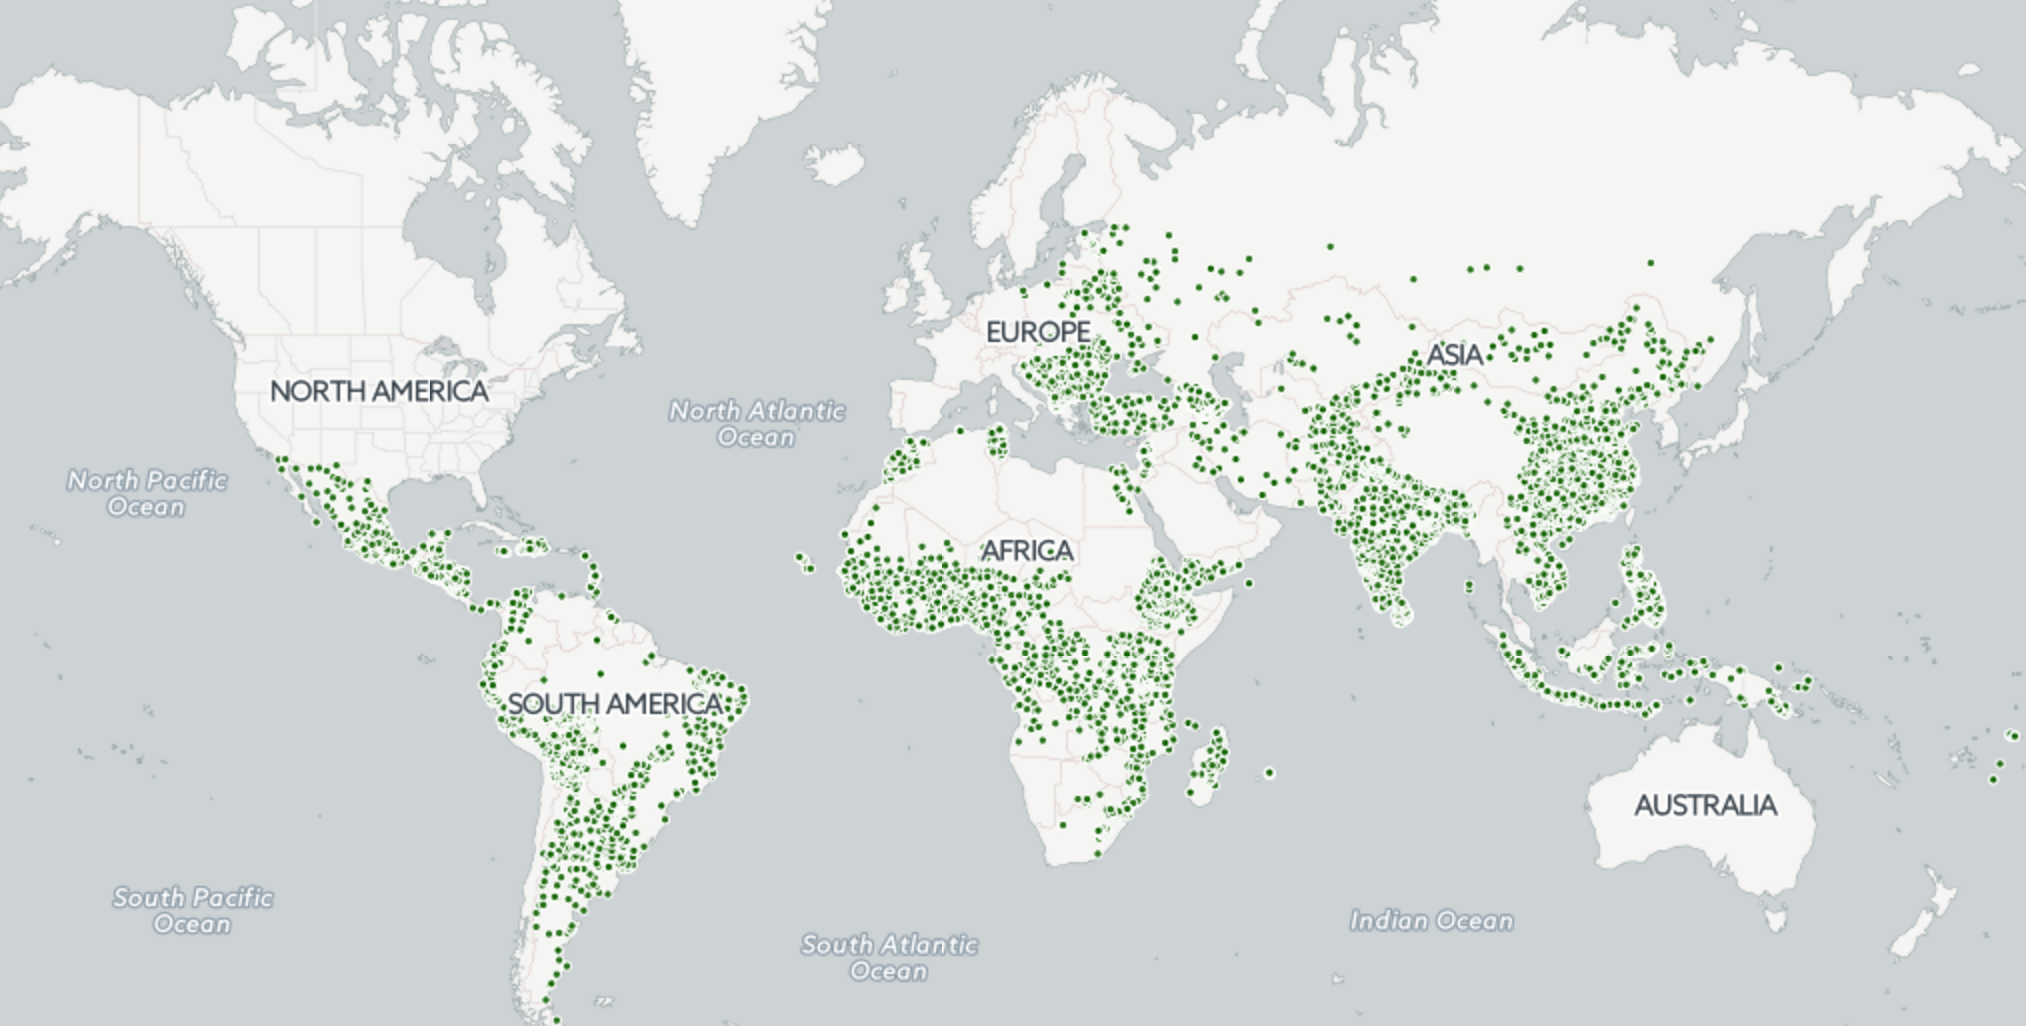
\includegraphics[width=\textwidth]{figs/wbprojects.png}
	\caption{world bank projects} \label{fig:wbprojects}
\end{figure}

For any serious human activity, there is the natural question: what difference does it make? 
Identifying and quantifying causal effects from data is one of the most interesting  research problem across many disciplines. 
For example, this arises in measuring the effectiveness of a drug in medical studies, in measuring the impact of changes in an e-commerce website design on customers, in evaluating the effectiveness of public policies. In our case, the world bank is interested in measuring the impact of aid projects it funded and supported all over the world over 30 years. 

The world bank's overarching goal is in economic development;  it formulates this as to "end extreme poverty by decreasing the percentage of people living on less than \$1.90 a day to no more than 3\%"  and to "promote shared prosperity by fostering the income growth of the bottom 40\% for every country" \cite{worldbankwebsite}. At an abstract level, the world bank provides funding for aid projects and can rely on a metric of choice to measure differences before a project begins and after a project ends. 
At the level of an individual project, we face the general crux of all observational studies, i.e., we can not observe the exact same geographic, environmental, social, economic, and historical setting with or without the project. So for measuring a difference, one has to rely on making meaningful comparisons between locations that are sufficiently similar. In addition to that, the world bank's operation is large scale with a large number of projects and worldwide, which creates a huge variability in the specific kind of project, the project's size, location, socio-economic, environmental, and historical setting. Figure \ref{fig:wbprojects} shows the locations of a set of world bank projects with 1168 projects in 16415 locations  that were performed between 2001 and 2012 on a global map.

The research questions, we investigate in this paper are:
\begin{itemize}
\item Can we estimate the impact of a project?
\item Can we identify subsets of entities in our data set that are meaningful to compare?
\item Can we identify attributes that are indicative of projects that show a positive (or negative) impact?
\end{itemize}

To do so, we enhance a given data set of world bank projects with additional information about the geographic, environmental, and economic 
characteristics over a number of years and rely on state-of-the-art techniques to estimate heterogenous causal effects. 
In our case, it is not interesting to estimate the overall average effect of all aid projects, but to identify subsets of projects by attributes and estimate average effects for individual subsets.
%Instead of investigate the causal effects for the whole population, in this paper, we are interested in estimating heterogeneous causal effects for subpopulations by features or covariates. We can estimate heterogeneity by covariates on causal effects and then conducting inference for a distinct unit.\\
%To avoid getting extreme treatment effects which lead to a spurious heterogeneous result, in disciplines such as clinical trial, they use pre-planed subgroup to analyze, for economic, they have pre-analysis plans for randomized experiments. With a data driven approach, the advantage is to discover some other causal effects instead of only the pre-planed subgroups.\\
To estimate heterogenous causal effects, there are several candidates, such as classification and regression trees  \cite{Breiman:2001:RF:570181.570182}, random forests \cite{breiman1984classification}, LASSO \cite{Tibshirani94regressionshrinkage}, and support vector machines (SVM) \cite{Vapnik1998}. 
%In this paper, we use the regression tree, the other methods such as random forest is also good candidate, but we focus on the regression tree in this paper.\\
In this paper, we follow the work of Athey and Imbens \cite{1504.01132} who demonstrated how regression trees and in conclusion also random forests can be adjusted to estimate heterogenous causal effects. It is based on the Rubin Causal Model or potential outcome framework where causal effects are comparisons between observed outcomes and counterfactual outcomes one would have observed under the absence of an aid project \cite{Imbens:2015:CIS:2764565}. Regression trees and random forests in traditional machine learning rely on training with data with known outcomes. Athey and Imbens showed that one can estimate the conditional average treatment effect on a  subset with regressions trees after an appropriate data transformation using propensity scores. This leads to the notion of transformed-outcome trees and causal trees that we use for our analysis. 

The rest of the paper is structured as follows. In Section 2, we recall the basic methodology for the calculation of transformed-outcome trees, causal trees, and random forests.  Section 3 introduces the data set, its characteristics, preprocessing steps and the calculation of propensity scores. In Section 4, we present the outcome of the analysis. We conclude in Section 5.
%In tradition, we can use decision trees to do prediction using the trained data or labeled data. We can build the regression tree to predicting the causal effects with the features as nodes in the tree. However, for the causal inference, the challenge is we do not have such data,in rubin causal model \cite{Imbens:2015:CIS:2764565}, we can only have the treated data or untreated data, but not both at the same time, hence we do not know the ground truth for prediction. We can't follow the traditional supervised machine learning method that we contract the tree with the trained the data and then use the the test data to do prediction based on the constructed tree. Follow the work of Athey and Imbens \cite{1504.01132}, we use causal tree to do heterogeneous causal effects estimation. However, in practice,for example in our case the world bank data set, within a node, there maybe only treated or untreated data, we will discuss in the paper how to explain such data and other issues \\
%\begin{itemize}
%\item first analysis on heterogeneous causal effect of world bank aid projects using machine learning method
%\item 
%
%\end{itemize}

\section{Methodology}

\subsection{Conditional average treatment effects}

Suppose we have a data set with n independently and identically distributed (iid) units with $ i = 1, \cdots, n$, for each unit, it has a feature vector $X_{i}  \in [0,1]^d$, a response $Y_{i} \in \mathbb{R}$ and treatment indicator $W_{i} \in \{0,1\}$.\\
For a unit-level causal effect, we can use the Rubin causal model and consider the treatment effect on unit $i$ being
$\tau_{i} = Y_{i}(1) - Y_{i}(0)$. 
%to estimate the average causal effect as %shown in function \ref{eq:1},
%\begin{equation} \label{eq:1}
%\tau_{i} = Y_{i}(1) - Y_{i}(0) \\
%\end{equation}
In this paper, we are interested in calculating the heterogenous causal effect, which we define as
$\tau(x) = \mathbb{E} \big[{Y_{i}(1) - Y_{i}(0) \mid X_{i} = x}\big]$ following \cite{RePEc:ecm:emetrp:v:71:y:2003:i:4:p:1161-1189}.
%as \ref{eq:2}, this estimator is proposed by \cite{RePEc:ecm:emetrp:v:71:y:2003:i:4:p:1161-1189},
%\begin{equation} \label{eq:2}
%\tau(x) = \mathbb{E} \big[{Y_{i}(1) - Y_{i}(0) \mid X_{i} = x}\big]\\
%\end{equation}
Of course, in an observational study, a unit is either untreated or not, so we know either $Y_{i}(0)$ or $Y_{i}(1)$ but not both. However,  one can still estimate $\tau(x)$ if one assumes unconfoundedness:
\begin{equation} \label{eq:3}
W_{i} \perp \left( Y_{i}(1), Y_{i}(0) \right)  \mid X_{i}\\
\end{equation}
Under the unconfoundedness assumption, Athey and Imbens \cite{Athey} show that one can estimate the causal effect as 

\begin{equation}\label{eq:3.5}
\tau(x) = \mathbb{E} \big[   Y^{*} \mid X_{i} =  x\big] 
\end{equation}
where the transformed outcome $Y^{*}$  is defined as
\begin{equation} \label{eq:4}
%Y_{i}^{*} =  Y_{i}^{obs} \cdot \frac{W_{i} - e(X_{i})}{e(X_{i}) \cdot (1 - e(X_{i}))} \\
Y_{i}^{*} =  Y_{i} \cdot \frac{W_{i} - e(X_{i})}{e(X_{i}) \cdot (1 - e(X_{i}))} 
\end{equation}
%
% is function \ref{eq:4}, 
and the propensity score function $e(x)$ is defined as $e(x)= \mathbb{E} \big[  W_{i} \mid X_{i} =  x \big]$.
%Function $e(x)$ is function \ref{eq:4.5}, to estimate the propensity score, 
%
Several approaches to estimate the propensity score are known \cite{rose:rubi:cent:1983}, \cite{HoImaKin07} including logic regression which we decided to use in this paper.
%%
%
%\begin{equation}\label{eq:4.5}
%e(x) = \mathbb{E} \big[  W_{i} \mid X_{i} =  x \big]
%\end{equation}

\subsection{Transformed Outcome Tree}
The transformed outcomes tree is a regression tree with $Y^{*}$ instead of $Y$. As mentioned above, the transformed outcome is calculated with  (\ref{eq:4}), then we can use traditional regression tree method to estimate the causal effect as 
$\tau(x) = \mathbb{E} \big[   Y^{*} \mid X_{i} =  x\big] $ based on the average transformed outcome of all nodes in the leaf of the tree where $i$ resides in.

\subsection{Causal Tree Model}
We use regression tree to estimate the heterogeneous causal effects, the first step is to construct the tree. To construct the regression tree, we recursively partition the node until the size of the node is less than a threshold we set or the gain of split is negative.\\
In classic regression tree, mean square error (MSE) is often used to as the criterion for node splitting, the average value within the node is used as the estimator. Following Asthey and Imbens \cite{1504.01132}, we use (\ref{eq:5}) as the estimator and we calculate the error of the node by summing $Y_{i}^ {*}- \hat{\tau}(X_{i})$.
\begin{equation} \label{eq:5}
%\begin{split}
\hat{\tau}^{CT}(X_{i}) = \sum_{i:X_{i} \in \mathbb{X}_{l}}  Y_{i}^{obs} \cdot \frac{ W_{i} / \hat{e}(X_{i})  }{\sum_{i:X_{i} \in \mathbb{X}_{l}}  W_{i} / \hat{e}(X_{i})}  \\
 - \sum_{i:X_{i} \in \mathbb{X}_{l}}  Y_{i}^{obs} \cdot\frac{ (1 - W_{i}) / (1 - \hat{e}(X_{i}))  }{\sum_{i:X_{i} \in \mathbb{X}_{l}}  (1 - W_{i}) / (1 - \hat{e}(X_{i}))}
% \end{split}
\end{equation}

\subsection{Pruning the tree}

To avoid overfitting of the tree, we need to prune the tree. We use the minimal cost complexity pruning and we define it as \ref{eq:6}. $\alpha$ is the complexity parameter, with it we can construct the regression with the right size.
\begin{equation}\label{eq:6}
R_{\alpha}(T) = R(T) + \alpha \left|\tilde{T}\right|
\end{equation}
where R(T) is the resubstitution error estimate of tree T, $\left|\tilde{T}\right|$ is defined as the complexity of the tree, which is the number of leaves in the tree,\\
To estimate the error of a node, we use function \ref{eq:7},
\begin{equation}\label{eq:7}
R(t) = \sum_{i=1}^{N}(Y_{i} - \hat{\tau}(X_{i}))
\end{equation}
where N is the total units in the nodes. \\

To get a sequence of $\alpha$, we minimize function \ref{eq:8},
\begin{equation}\label{eq:8}
g(t,T) = \frac{R(t) - R(T_{t})}{\left|\tilde{T_{t}}\right| - 1}
\end{equation}
where $T_{t}$ is a subtree of T rooted at node t.\\
We use the weakest link cutting to determine $\alpha$ and use it as the complexity parameter when we build the tree for the whole data set. \\
We use the train data set to construct the tree and then apply weakest link cutting to the tree with $\alpha$ starting with 0. Until there is one node in the tree, we get a series of
$\alpha$, $ \alpha_{0} < \alpha_{1} < \cdots < \alpha_{k}$.
Then we set $\beta_{0} $ = 0, $\beta_{1} = \sqrt{\alpha_{1}\alpha_{2}}$, $\cdots $, $\beta_{k-1} = \sqrt{\alpha_{k-1}\alpha_{know}}$

We use V-fold cross validation to estimate the errors for different $\beta$ and use the $\beta$ with minimum error.
We divide the data into k sets randomly with the same size, we use $1,2,3,\cdots,v-1,k$ to represent the v-th data part and (k) as the left part of the data correspond to the v-th part. For each $\beta_{k}$, we useV-fold cross validation to get the estimated error. The error is calculated by function \ref{eq:10},
 \begin{equation}\label{eq:10}
Err(\beta;Y_{i}^{v}, X_{i}^{v}) =  \sum_{1}^{N}(Y_{i}^{v} - \hat{\tau}(X_{i}^{(v)}))
\end{equation}
where $N = n/V$, n is the size of the whole data set. 
We can then calculate error $R(T(\beta)) $for each $\beta$ value as the average error:
\begin{equation}\label{eq:9}
R(T(\beta)) = \frac{1}{V}\sum_{1}^{V}Err(\beta;Y_{i}^{v}, X_{i}^{v})
\end{equation}

\subsection{Random forest with TOT trees}












\section{Data}

\subsection{Data sources and collection}
We leverage the following data sources in this analysis:
\begin{table*}[t]
\begin{center}
  \begin{tabular}{| p{3cm} | p{5cm} | p{6cm} |}
    \hline
    Variables &  Description & Source \\ \hline
    Forest Cover& NASA Long Term Data Record measurements of vegetative cover & \url{http://ltdr.nascom.nasa.gov/cgi-bin/ltdr/ltdrPage.cgi }\\ \hline
    World Bank Project Locations & Double-blind geocoded information on the geographic location of each World Bank project & \url{http://aiddata.org/level1/geocoded/worldbank} \\ \hline
    Distance to Rivers & The calculated average distance to all rivers & \url{http://hydrosheds.cr.usgs.gov/index.php} \\ \hline
    Distance to Commercial Rivers & Calculated average distance to all commercial rivers & \url{http://hydrosheds.cr.usgs.gov/index.php}  \\ \hline
    Distance to Roads &  Distance to nearest road & \url{http://sedac.ciesin.columbia.edu/data/set/groads-global-roads-open-access-v1}\\ \hline
    Elevation & Elevation data measured from the Shuttle Radar Topography Mission & \url{http://www2.jpl.nasa.gov/srtm/}\\ \hline
    Slope&  Slope data calculated based on the Shuttle Radar Topography Mission & \url{http://www2.jpl.nasa.gov/srtm/}\\ \hline
    Accessibility to Urban Areas & European Commission Joint Research Centre estimation of urban travel times. & \url{http://forobs.jrc.ec.europa.eu/products/gam/download.php}\\ \hline
    Population Density & Center for International Earth Science estimation of population density, derived from Nighttime Lights & \url{http://sedac.ciesin.columbia.edu/data/collection/gpw-v3}  \\ \hline
    Air Temperature & University of Delaware Long term, global temperature data interpolated from weather station measurements. &\url{http://climate.geog.udel.edu/~climate/ }\\ \hline
    Precipitation & University of Delaware Long term, global precipitation data interpolated from weather station measurements.& \url{http://climate.geog.udel.edu/~climate/}\\ 
    \hline
    
  \end{tabular}
  \caption{Covariates of the data sets for World Bank projects}
  \label{table:data}
\end{center}
\end{table*}
    
\subsection{Data pre-processing}
  This analysis uses three key types of data: satellite data to measure vegetation, data on the geospatial locations of World Bank projects, and covariate datasets (the sources of which are detailed above). 
Our primary variable of interest is the fluctuation of vegetation proximate to World Bank projects, which is derived from long-term satellite data (NASA 2015). 
There are many different approaches to using satellite data to approximate vegetation on a global scale, and satellites have been taking imagery that can be used for this purpose for over three decades.  
Of these approaches, the most frequently used is the Normalized Difference Vegetation Index (NDVI).  The NDVI is a metric that has been used since the early 1970s, and is one of the simplest and most frequently used approaches to approximating vegetative biomass.  
NDVI measures the relative absorption and reflectance of red and near-infrared light from plants to quantify vegetation on a scale of -1 to 1, with vegetated areas falling between ~0.2 and 1. 
The reflectance by chlorophyll is correlated with plant health, and multiple studies have illustrated that it is generally also correlated with plant biomass. 
In other words, healthy vegetation and high plant biomass tend to result in high NDVI values (Dunbar 2009).  
Using NDVI as an outcome measure has a number of other benefits, including the long and consistent time periods for which it has been calculated.  
While the NDVI does have a number of challenges - including a propensity to saturate over densely vegetated regions, the potential for atmospheric noise (including clouds) to incorrectly offset values, and reflectances from bright soils providing misleading estimates - the popularity of this measurement has led to a number of improvements over time to offset many of these errors.  
This is especially true of measurements from longer-term satellite records, such as those used in this analysis, produced from the MODIS and AVHRR satellite platforms (NASA 2015).
\par
The second primary dataset used in this analysis measures where - geographically - World Bank projects were located.  This dataset was produced by AidData (2016), relying on a double-blind coding system where two experts employ a defined hierarchy of geographic terms and independently assign uniform latitude and longitude coordinates, precision codes, and standardized place names to each geographic feature. If the two code rounds disagree, the project is moved into an arbitration round where a geocoding project manager reconciles the codes to assign a master set of geocodes for all of the locations described in the available project documentation. This approach also captures geographic information at several levels?coordinate, city, and administrative divisions?for each location, thereby allowing the data to be visualized and analyzed in different ways depending upon the geographic unit of interest. Once geographic features are assigned coordinates, coders specify a precision code that varies from 1 (exact point) to 9 (national-level project or program).
AidData performs many procedures to ensure data quality, including de-duplication of projects and locations, correcting logical inconsistencies (e.g. making sure project start and end dates are in proper order), finding and correcting field and data type mismatches, correcting and aligning geocodes and project locations within country and administrative boundaries, validating place names and correcting gazetteer inconsistencies, deflating financial values to constant dollars across projects and years (where appropriate), strict version control of intermediate and draft data products, semantic versioning to delineate major and minor versions of various geocoded datasets, and final review by a multidisciplinary working group. 
\par
In addition to the project name, the World Bank provided information on donors and amounts of funding for each project.
For a subset of project, there is data on the performance evaluation of projects for evaluating effectiveness of staff. 
We also learnt that a single project rarely resides on a single location. It typically spreads out over a number of n locations with typical values of $n=2$ but ranging up to $n=10$.

\subsection{Data characteristics}
For variables listed in the Table \ref{table:data} excluding the geographic location, population density and NDVI, we have minimum, maximum, and average values for each year between 1992 and 2012. For NDVI and population density, we only have a time series with average annual values. The project's geographic location is assumed constant. While annual values for covariates such as elevation and slope are typically constant over time, for others we expect to see change over time, in particular those in response to economic development such as distance to roads, accessibility to urban areas and population density. Air temperature and precipitation describe environmental conditions that may change subject to long-term trends due to a change in climate, subject to multi-year seasonal effects due to the El Nino Southern Oscillation, and subject to local or regional environmental changes, e.g. a massive deforestation. For lack of space, we only describe some characteristics of NDVI data.
Figure \ref{fig:ndvi} a) shows average annual NDVI values of all project locations for each year since 1982. The mean values are non-negative for all projects over all years and typical values are around 0.2 which is a lower bound for areas with vegetation.
For each project location, the average annual NDVI values give a time series for which we can do a linear regression fitting to estimate the slope of an underlying trend. Figure \ref{fig:ndvi} b) shows the distributions of slope values for a time series of NDVI values that starts in 1982 and ends with the year before the project starts. We see that regardless of the year the projects start, more than 75\% of all projects face a starting situation where NDVI values are slightly on the rise.

\begin{itemize}
%\item provide an overview of the total number of covariates and their characteristics. As in table \ref{table:data}, the main covariates are in the table, for temperature, precipataion, they both have data for 20 years including maximum, minimum,average value of each year, also the NDVI values and avg light percentage value for 20 years but only contains average value. There are also some other covariates that not in the table, such as project name, the donors, the fund of the projects, we refer people who interest in the data to aiddata website for details. 
%\item Forest cover (= NDVI?): time series. As this is an important variable, can we get a box plot with mean values and slope values for all projects? 
\item for covariates, we should provide some outline about type (categorical, ordinal,numerical), ranges of values, and if some normalization is applied. If data gives a time series, its granularity (time and space), concerns about precision
(no space for too much details about the data, we can refer them to aiddata website for details)
\item set of world bank projects covers a broad range of topics and individual projects do not necessarily directly target deforestation. We want to recognize projects that show an impact on forest cover, be it positive or negative. (too many projects to check, can only guess from the title)
\item discuss projects and project locations: a project can take place at more than one geographic location.( The data contains projects that have between 1 and 10 locations. )  One project may contains sub projects in different locations from one to hundreds.  This raises the question on how to aggregate average treatment effects across a set of project locations into a single value for the overall project.
\end{itemize}


\begin{figure}
	\subfloat[]{  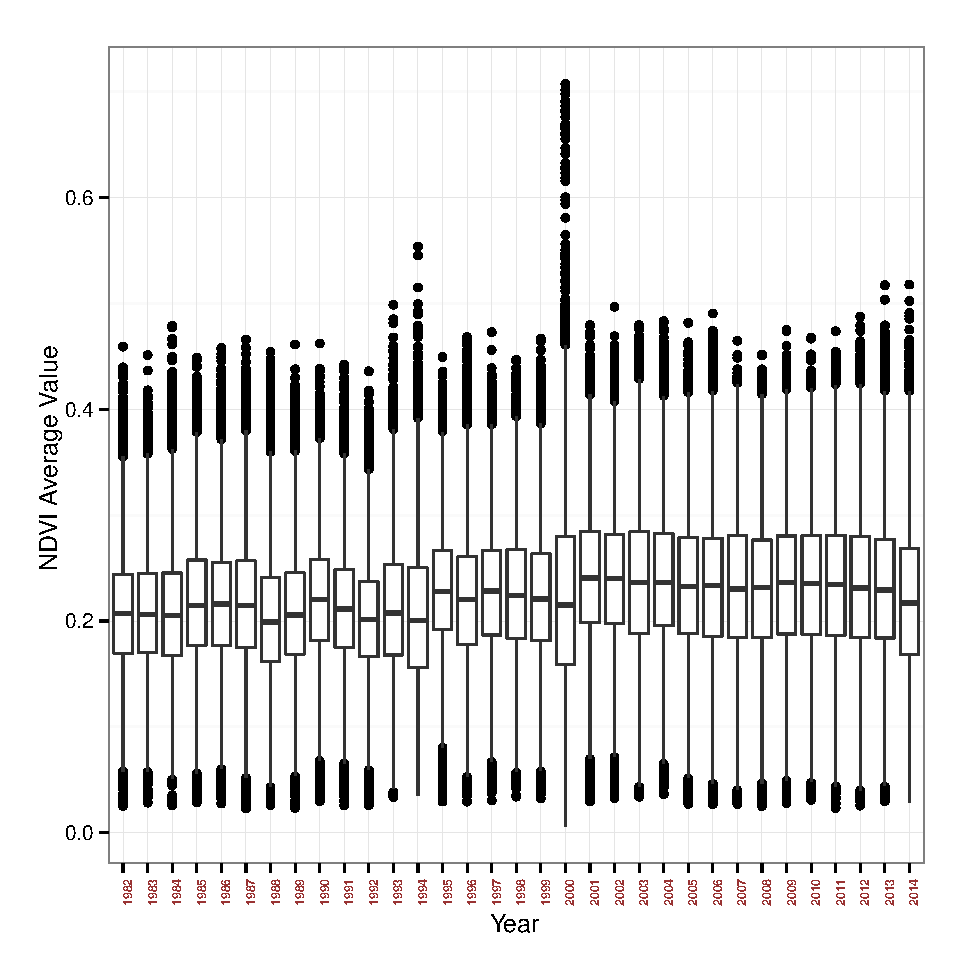
\includegraphics[width=0.5\textwidth]{figs/ndvi.eps}}	
	\subfloat[]{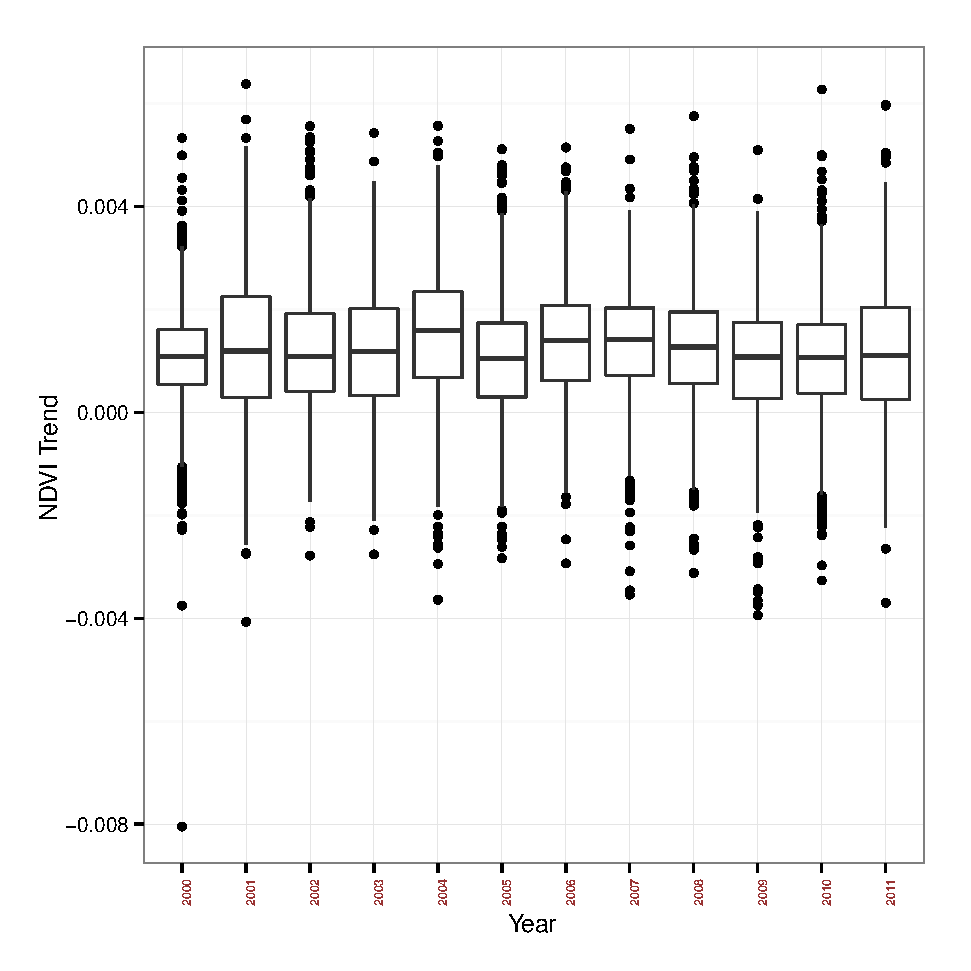
\includegraphics[width=0.5\textwidth]{figs/ndvitrend.eps}}	
	\caption{NDVI features of all the projects} \label{fig:ndvi}
\end{figure}


\subsection{Data interpretation for the context of measuring heterogenous treatment effects}
CT and TOT methods expect a separation of the data set into treated and untreated cases.
A treatment in our setting is of course the fact that a project takes place. As our data set only contains project data, we make the assumption that the observed treatment effect should positively correlate with the amount of funding, i.e. huge amounts of funding are expected to have a bigger effect than small amounts of funding. In this way, we assign $W_i=1$ if a project's funding exceeds a fixed threshold of \$ xxx.
The data set contains 1168 projects in 16415 locations that were performed between 2001 and 2012. Many covariates are described with time series data which leads to the question on how to compare projects that started in different years. One possibility is to retain absolute values for points in time, i.e. precipitation in 2002, which has the benefit to keep numerical comparisons of actual precipitation values across projects meaningful (if that year was a draught season in a large region) but creates the difficulty that projects have a variable set of features as we can not include covariates for the time after the project begins. Another possibility is to use time stamps relative to the project start, i.e. have values for $1,2,3,...,k$ years before the project starts. The benefit is that all units can share the same set of covariates (after some truncation), but for example the comparison of values for precipitation 3 years before a project stars across some projects may ignore hidden global constraints. This effect gets more pronounced if one compares the outcome, the NDVI values for years following the project, in the computation of the response $Y$. A further option is to aggregate time series data into fewer features, e.g. to represent it by a linear model and use intercept and slope.
This incorporates further assumptions and shares the same issues mentioned before for relative time stamps. 
In order to avoid this issue, we decided to focus on a subset of projects that all started in the same year. We selected the year 2004.
As a single project typically takes place at several project locations, we decided to consider each project location as an individual unit. 
This means, the overall data set of 114 projects that started in 2004 at a total of 1628 project locations gives $n=1628$ units.
For the feature vector, we include longitude and latitude of the geolocation and time series data for other variables till the beginning of a project. As CT and TOT methods tolerate large numbers of covariates but can not perform functions such as average over a set of features, we decided to include annual values for time series data plus estimates of average and slope (as for example shown for NDVI in Fig. \ref{fig:ndvi}). The idea is to recognize if the analysis method has a preference for a particular year or for average or slope.
The total length of the feature vector is $d=XXX$. All covariates are numerical and their values are taken as is and not normalized. 
%The response $Y_i$ of a project location $i$ is the slope of a linear regression that we perform on annual average NDVI values for the years 2004 till 2010, i.e. six years from the beginning of the project.
Let $ndvi_i(92,03)$ denote the average of NDVI values observed for project location $i$ over the years from 1992 to 2003 before the project starts. Let $ndvi_i(05,12)$ describe the corresponding value for the eight years after the project starts.
%The response $Y_i = ndvi_i(05,12)-ndvi_i(92,03)$ of a project location $i$ is the difference of average NDVI values over six year periods before and after the beginning of the project.
The response $Y_i = ndvi_i(05,12)-ndvi_i(92,03)$ is the difference of the two averages.
In order to calculate $Y^\ast$ for $Y$, we need to obtain the propensity score $e(x)$, which describes the expected value for treatment $W_i$ for a given feature vector $x$. Note that the propensity score for each unit is calculated in a preprocessing step that is independent from the applied CT or TOT method. 

\begin{itemize}
\item describe how we calculate propensity scores: We use linear model to calculate the pscore. 
\end{itemize}
 



%\begin{itemize}
%\item general idea is to separate data into treated and untreated cases, there is no particular notion of time. For each entity (treated or untreated), a set of covariates are provided.
%\item in our case: we decided to interpret the project start as the treatment and the change in forest cover (average?, slope?) as the treatment effect. We use average before 1992-2003 for ndvi and 2005-2012.
%\item as we only have data for locations were a project takes place, we consider small scale projects with small amounts of funding as untreated cases (???)
%\item We decided for time series data: split into two parts, before and after project start. We only take covariates for data before project starts into account for selecting variables in the random forest construction. We use data after the project starts to compute treatment effects. Rationale: covariates with data after treatment may be correlated with the outcome which would corrupt the calculation of average treatment effects (?).
%\item Since large scale correlations and changes beyond the reach of the project such as the beginning or ending of a draught period over several years may by hiding within time series data, we decided to compare projects that all started in the same year in order to have level playing field for projects in the same geographic region.
%\end{itemize}
%
%\subsection{Calculation of Propensity Scores}
%\begin{itemize}
%\item describe how we calculate propensity scores before we feed the data into a random forest. We use linear model to calculate the pscore. 
%\end{itemize}



\section{Experiments}
In 2004, there are totally 114 projects contain 1628 subproject in different locations. 
\subsection{Software packages}
Our method is based on the R package rpart \cite{cart}. Rpart support user defined split function, therefore, we can use the split criterion function \ref{eq:5}. To improve the efficiency of the r program, we use rcpp and call C++ functions inside the split and evaluation function for each node in the tree. To further improve the c++ functions, we use openmp inside the C++ functions. To avoid the extreme cases, such as only treated or untreated data in the internal nodes, we would not split under in such condition. We use the randomForest \cite{rf} R package to build the forest.

\subsection{TOT Results}
\begin{itemize}
\item observation: calculation of $/alpha$ for pruning is computationally expensive but can be parallelized. This can be done for all methods. Discuss speed up for one of the methods.
\item Resulting average treatment effect obtained from leaf node. In order to have a reasonable estimate, there is a trade off in being specific (have a refined tree with little variation but fewer units per leaf node) or being more general and have more diverse units in a leaf node but a have more values to support an estimate for an average value
\item TOT allows us to compute average treatment effect for each unit $i$
\item TOT allows us to rank covariates according to the order of variables in the tree
\item TOT allows us to find similar projects to compare based on sets of units in each leaf
\item Can not measure how representative the tree, unclear how to measure confidence in judgement etc
\item discuss the actual outcome for a single example project that serves as an illustrating example all along the other methods (may be a particular good project)
\end{itemize}

\subsection{CT Results}
\begin{itemize}
\item Resulting average treatment effect obtained from leaf node. In order to have a reasonable estimate, one needs at least one treated and one untreated unit per leaf. In order to ensure this, one can configure the splitting rule accordingly, however this may come for the price that units remain in the same set that are not very similar.
\item CT allows us to compute average treatment effect for each unit $i$ if at least one treated, untreated unit is present
\item CT allows us to rank covariates according to the order of variables in the tree
\item CT allows us to find similar projects to compare based on sets of units in each leaf
\item Can not measure how representative the tree, unclear how to measure confidence in judgement etc
\item discuss the actual outcome for a single example project that serves as an illustrating example all along the other methods (may be a particular good project)
\end{itemize}

\subsection{Random Forest Results}
\begin{itemize}
\item Resulting average treatment effect obtained from averaging the outcomes of all TOT trees in the forest. 
\item RF allows us to compute average treatment effect for each unit $i$
\item RF allows us to rank covariates according to the order of variables in the tree and quantify this in terms of quantiles (percentage of trees that use covariate among its top k covariates or alike)
\item RF allows us to find similar projects to compare based on sets of units in each leaf (
\item Can not measure how representative the tree, unclear how to measure confidence in judgement etc
\item discuss the actual outcome for a single example project that serves as an illustrating example all along the other methods (may be a particular good project)
\end{itemize}

\subsection{Comparison}


\begin{itemize}
\item variable importance, important variables should be in the top levels of the tree, important to the causal effects
\item regression variability, interval, in a forest, how stable the effect of  a project is, if the variance is small, we can trust the result
\item validate the result, one of the challenges is we do not have golden truth for the projects, we have partial result from world bank IEG which is for the assessment of the implement of the overall projects, as each projects usually have more than two sub projects on different locations, the estimation is coarse. Another source of result is from the economist result,
based on these two evaluation, we can validate our work to some extent. 

\item About $83\%$ projects in 2004 have more than 1 locations, the IEG outcomes take all of the them as a whole, in our random forest, we have causal results for sub projects, hence, one project may have both good and bad causal effects.

\item quantile for each project location, variability of the causal effects, uncertainty of the result, $8\%$ data have all causal effects have same effect, either positive or negative result, $90\%$ have either positive or negative result from quantile $25\%$ to $75\%$
 
\end{itemize}



\begin{table*}[t]
	\begin{center}
		\begin{tabular}{l | c | c | c | c}
		\hline
			WB region 						& CT 			& TOT 			& RF 			& ECON \\ \hline
			AFRICA 							& -0.0034007384 	& -0.002259834  	& -0.002070222	& -0.037396489 \\ 
			EAST ASIA AND PACIFIC 			& -0.0004073951 	& -0.002602419	& -0.002338640 	& -0.054120740 \\ 
			EUROPE AND CENTRAL ASIA 		&-0.0077536156 	& 0.026434682		& 0.027010477 	& 0.030465111 	\\ 
			LATIN AMERICA AND CARIBBEAN		& 0.0089683258	& 0.014169258		& 0.010182891 	& -0.013437384 \\ 
			MIDDLE EAST AND NORTH AFRICA 	& -0.0025123259 	& -0.017290754	&-0.015723577 	& -0.008182447 \\ 
			SOUTH ASIA 						&-0.0096351385	& -0.010894742	& -0.010095676 	& -0.081190785 \\ \hline
		\end{tabular}
		\caption{causal effect by regions}\label{table:resbyregion}
	\end{center}
	
\end{table*}



\begin{figure}
	\subfloat[good projects rank]{  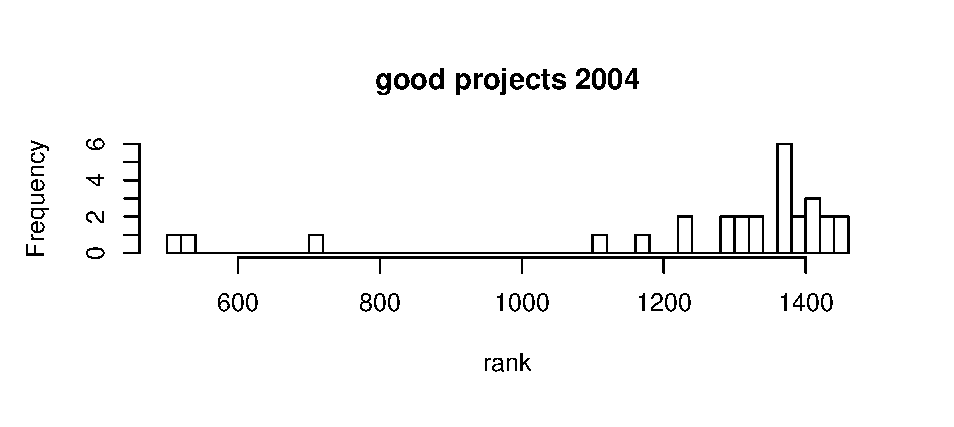
\includegraphics[width=0.3\textwidth]{figs/goodrank.eps}}	
	\subfloat[bad projects rank]{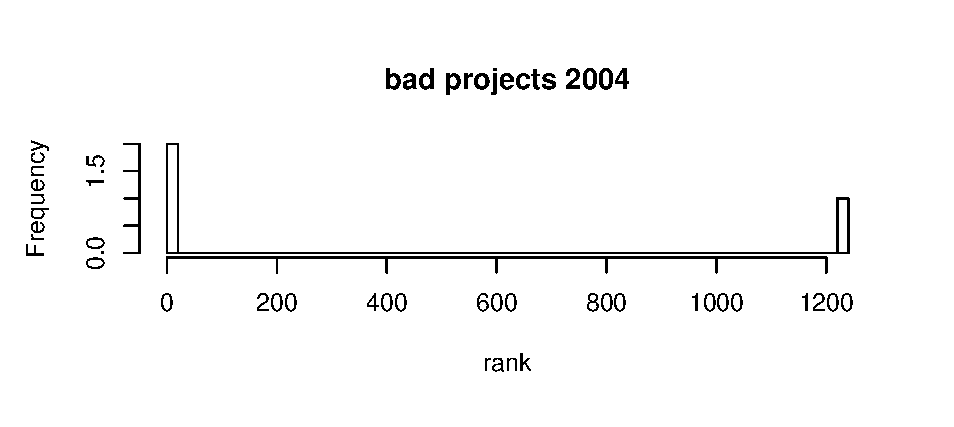
\includegraphics[width=0.3\textwidth]{figs/badrank.eps}}	
	\subfloat[moderate projects rank]{  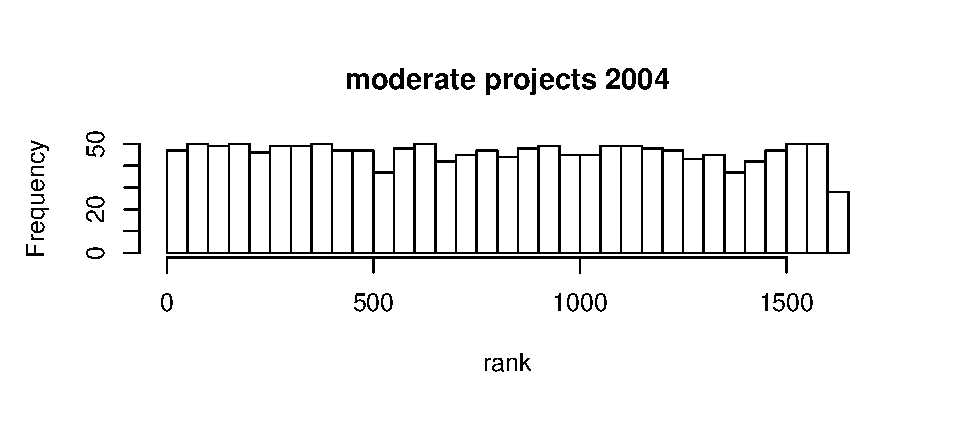
\includegraphics[width=0.3\textwidth]{figs/moderaterank.eps}}	
	\caption{original data without considering quantile}
\end{figure}



\begin{figure}
	\subfloat[Econ]{  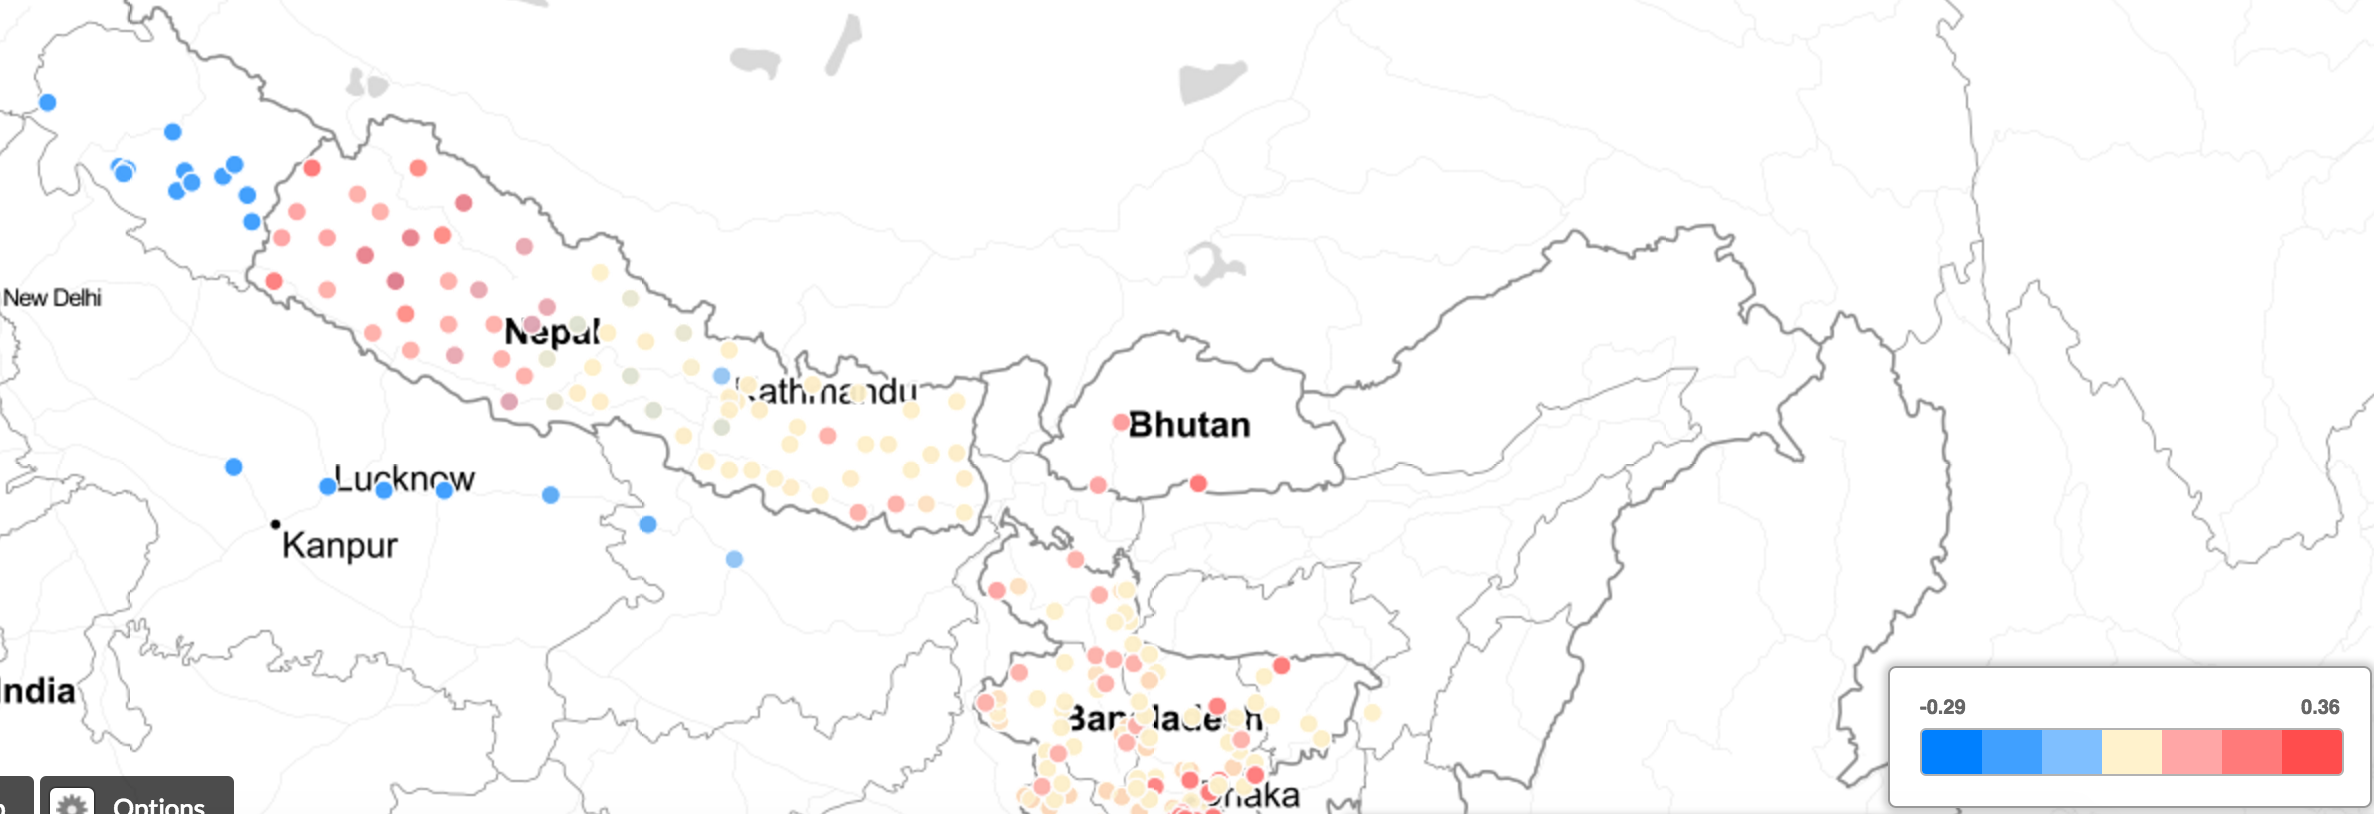
\includegraphics[width=0.35\textwidth]{figs/econmap.png}\label{fig:econ}}	
	\subfloat[Random Forest]{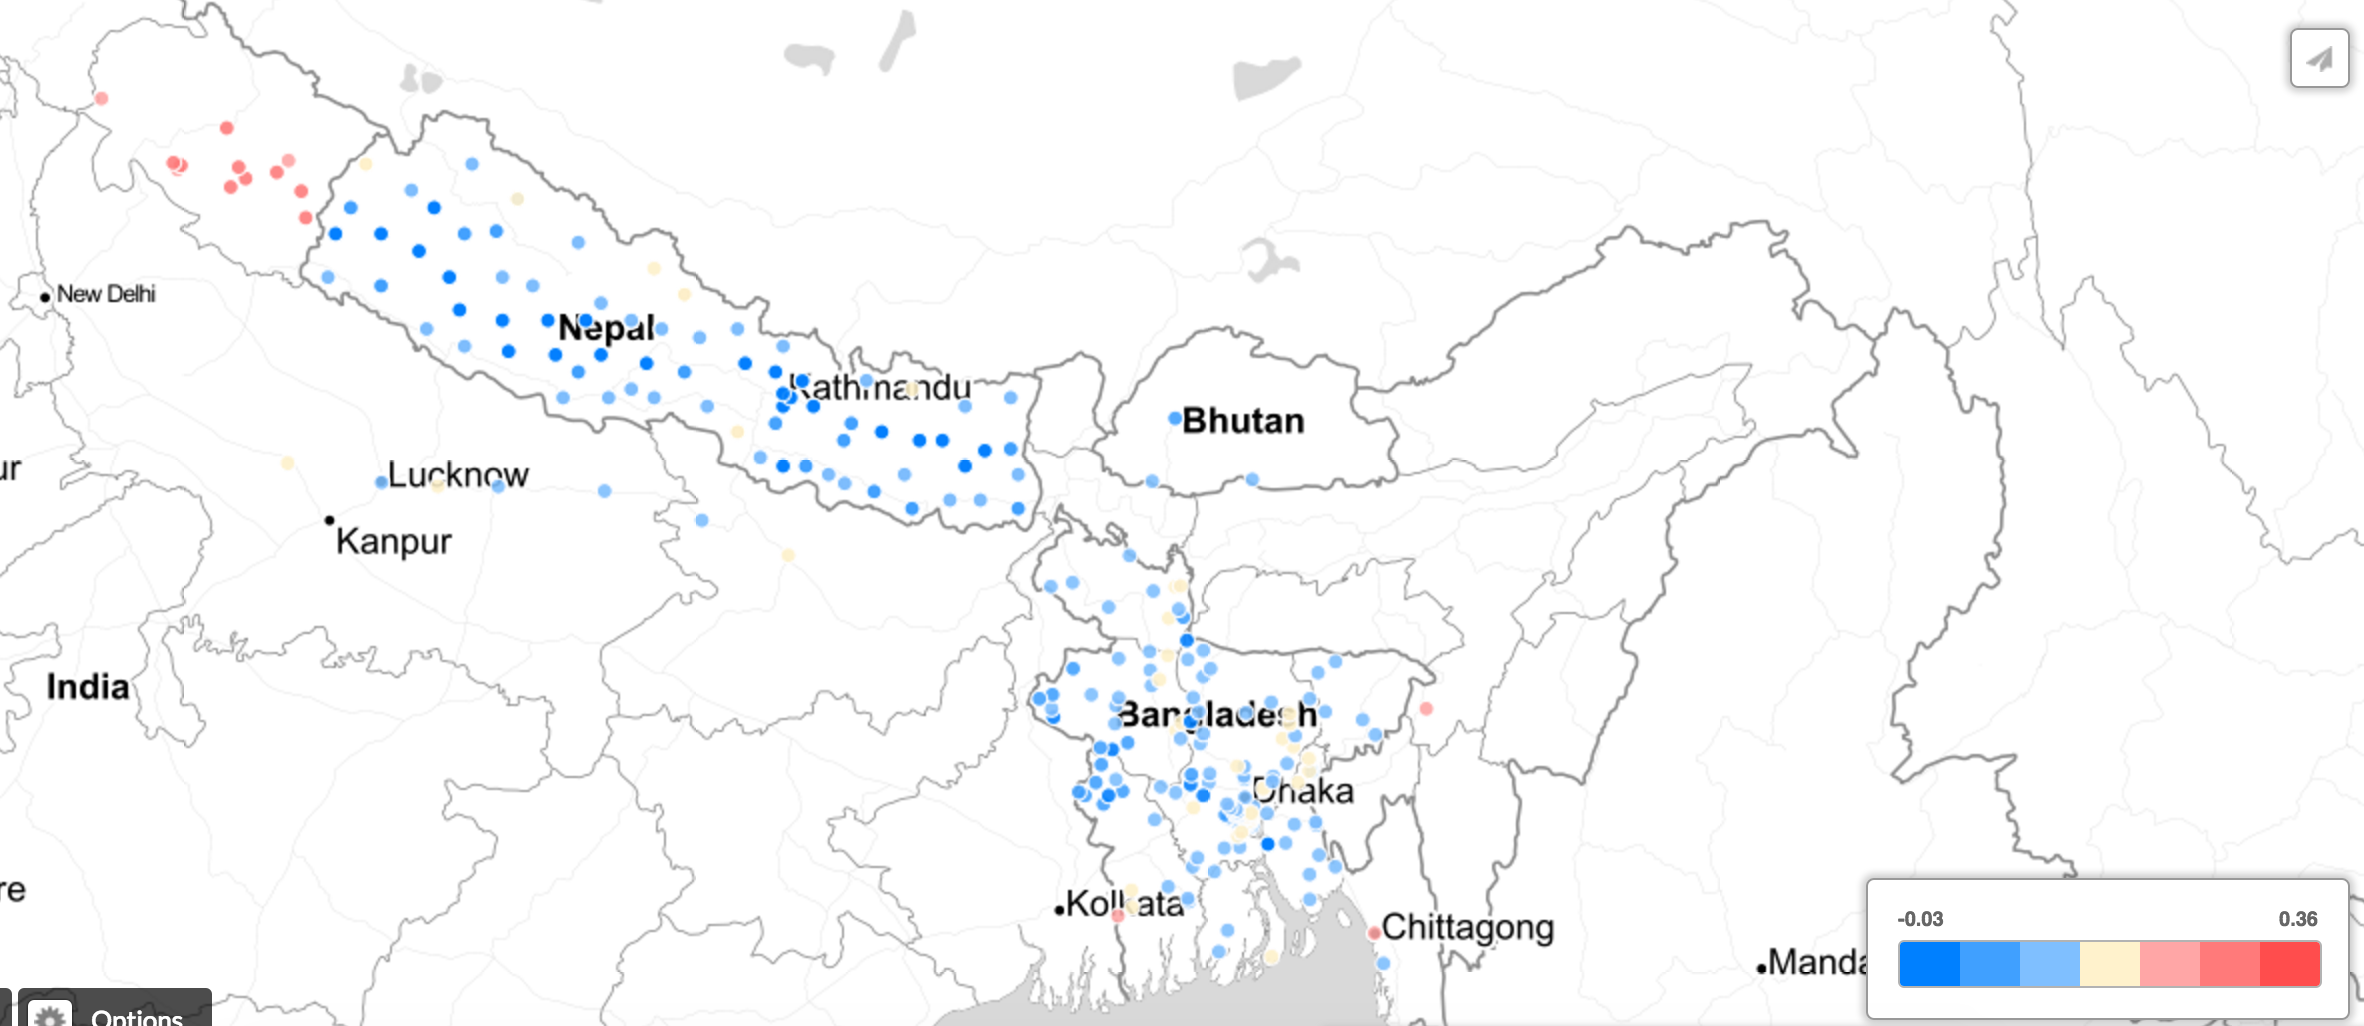
\includegraphics[width=0.35\textwidth]{figs/rfmap.png}\label{fig:rf}}	
	\subfloat[IEG outcome]{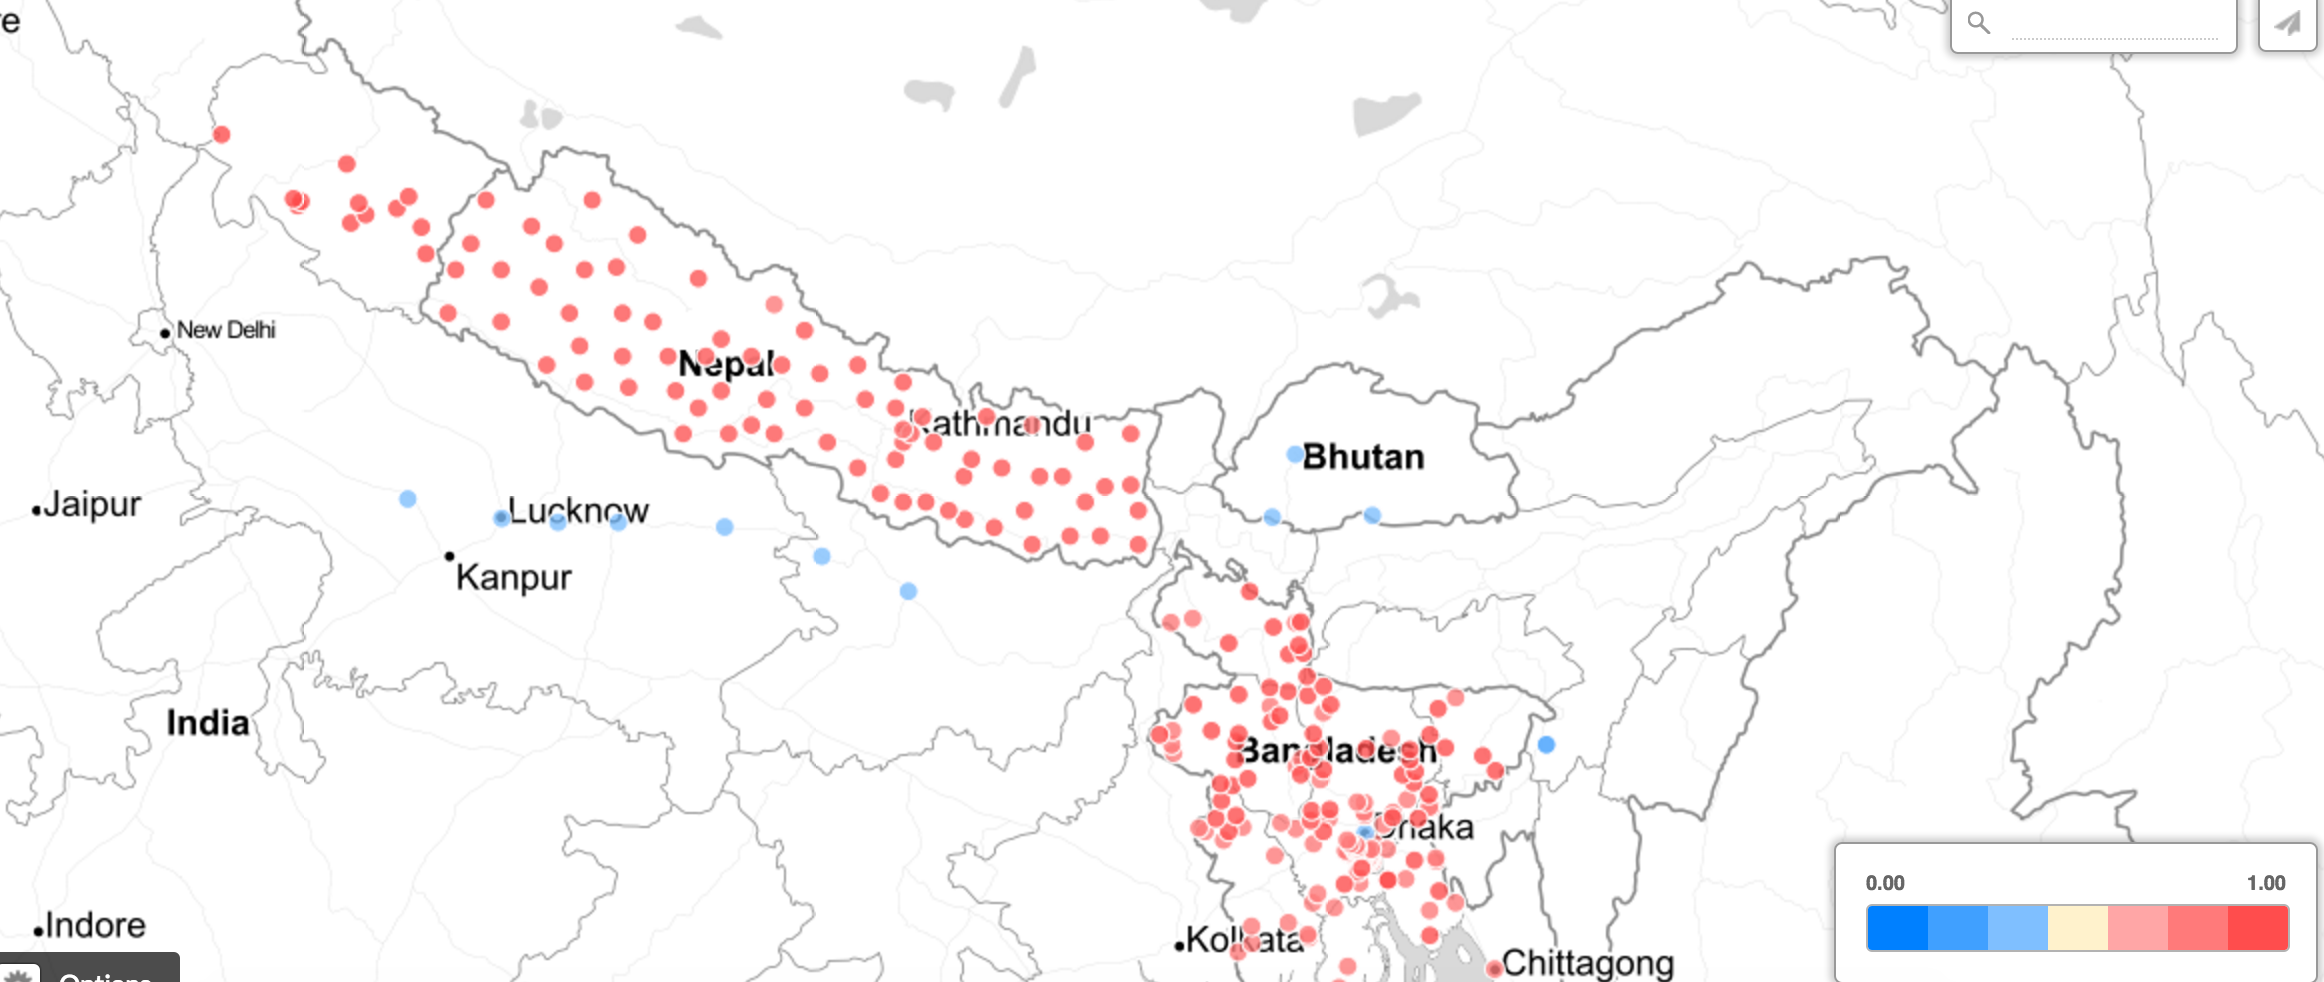
\includegraphics[width=0.35\textwidth]{figs/wbieg.png}\label{fig:ieg}}
	\caption{Nepal area 2004}
\end{figure}

\begin{figure}
	\subfloat[Econ]{  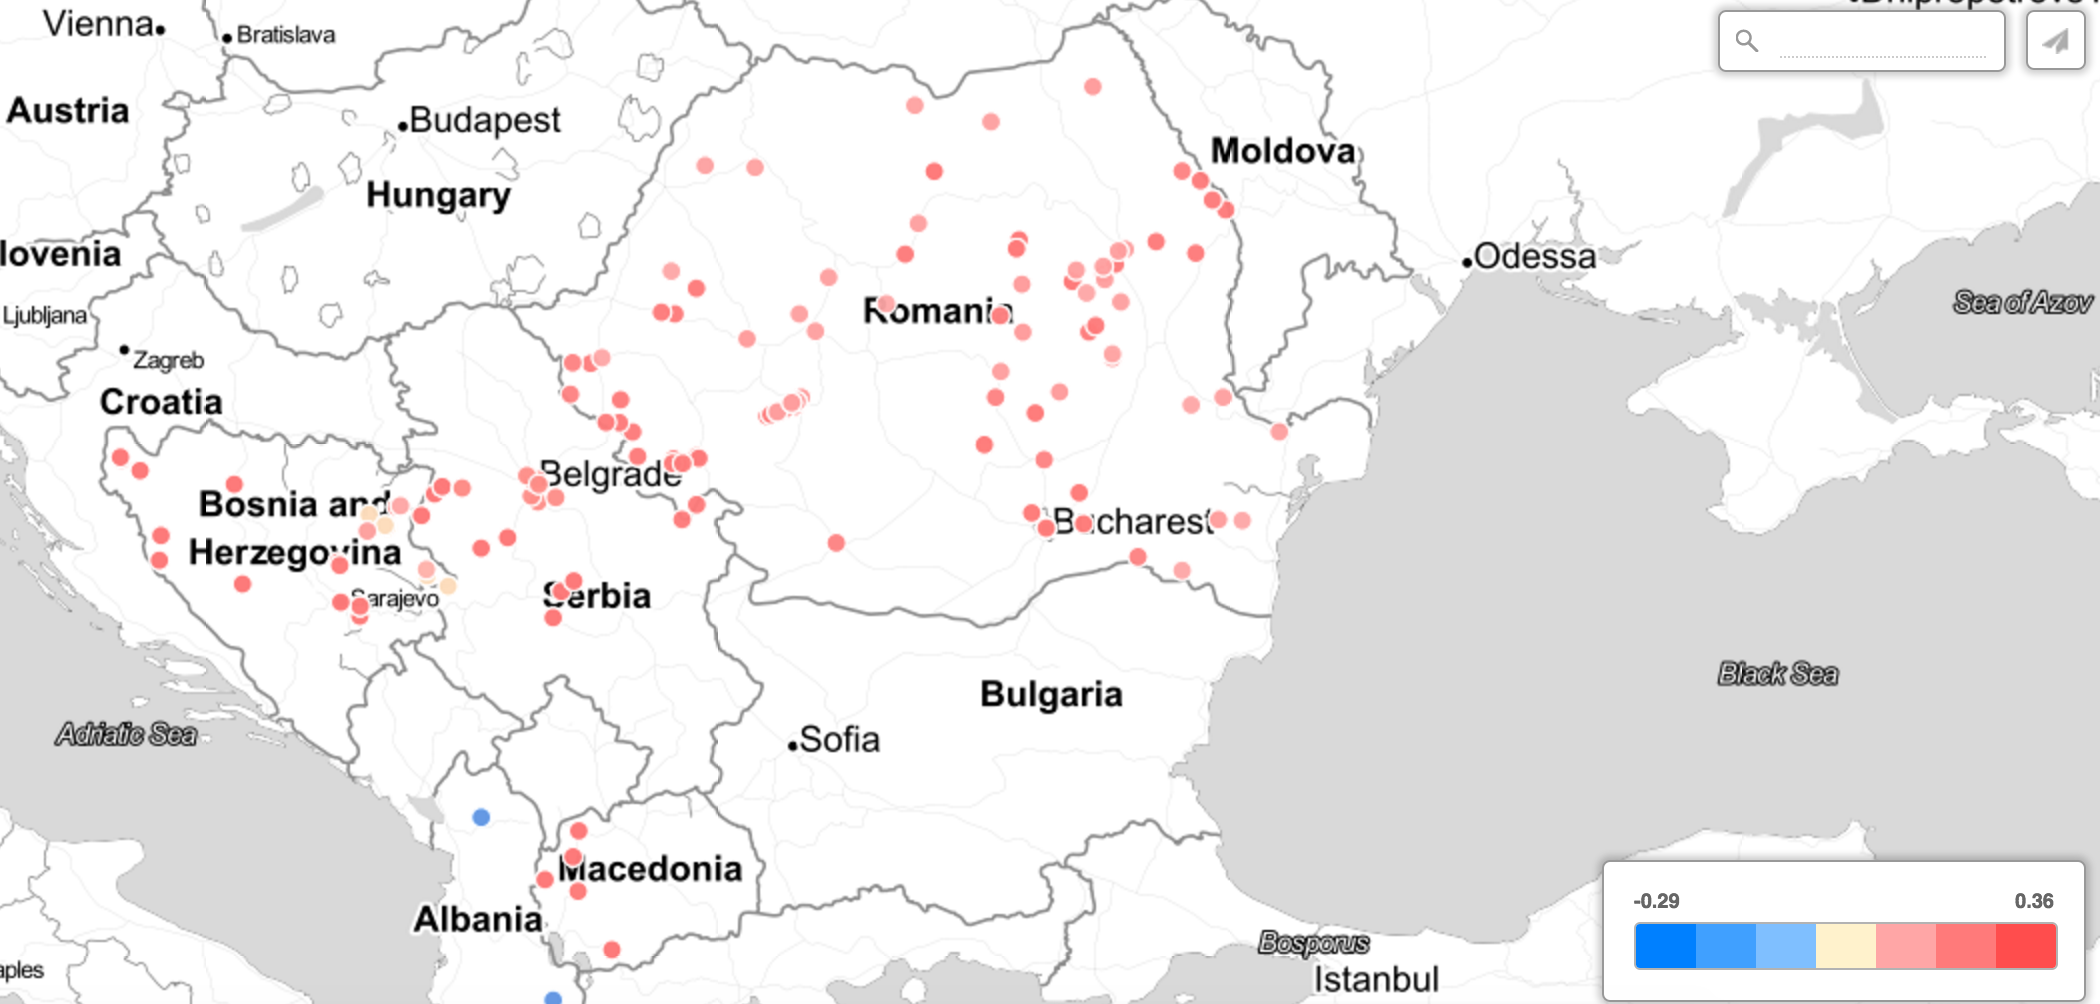
\includegraphics[width=0.35\textwidth]{figs/econeu.png}\label{figeu:econ}}	
	\subfloat[Random Forest]{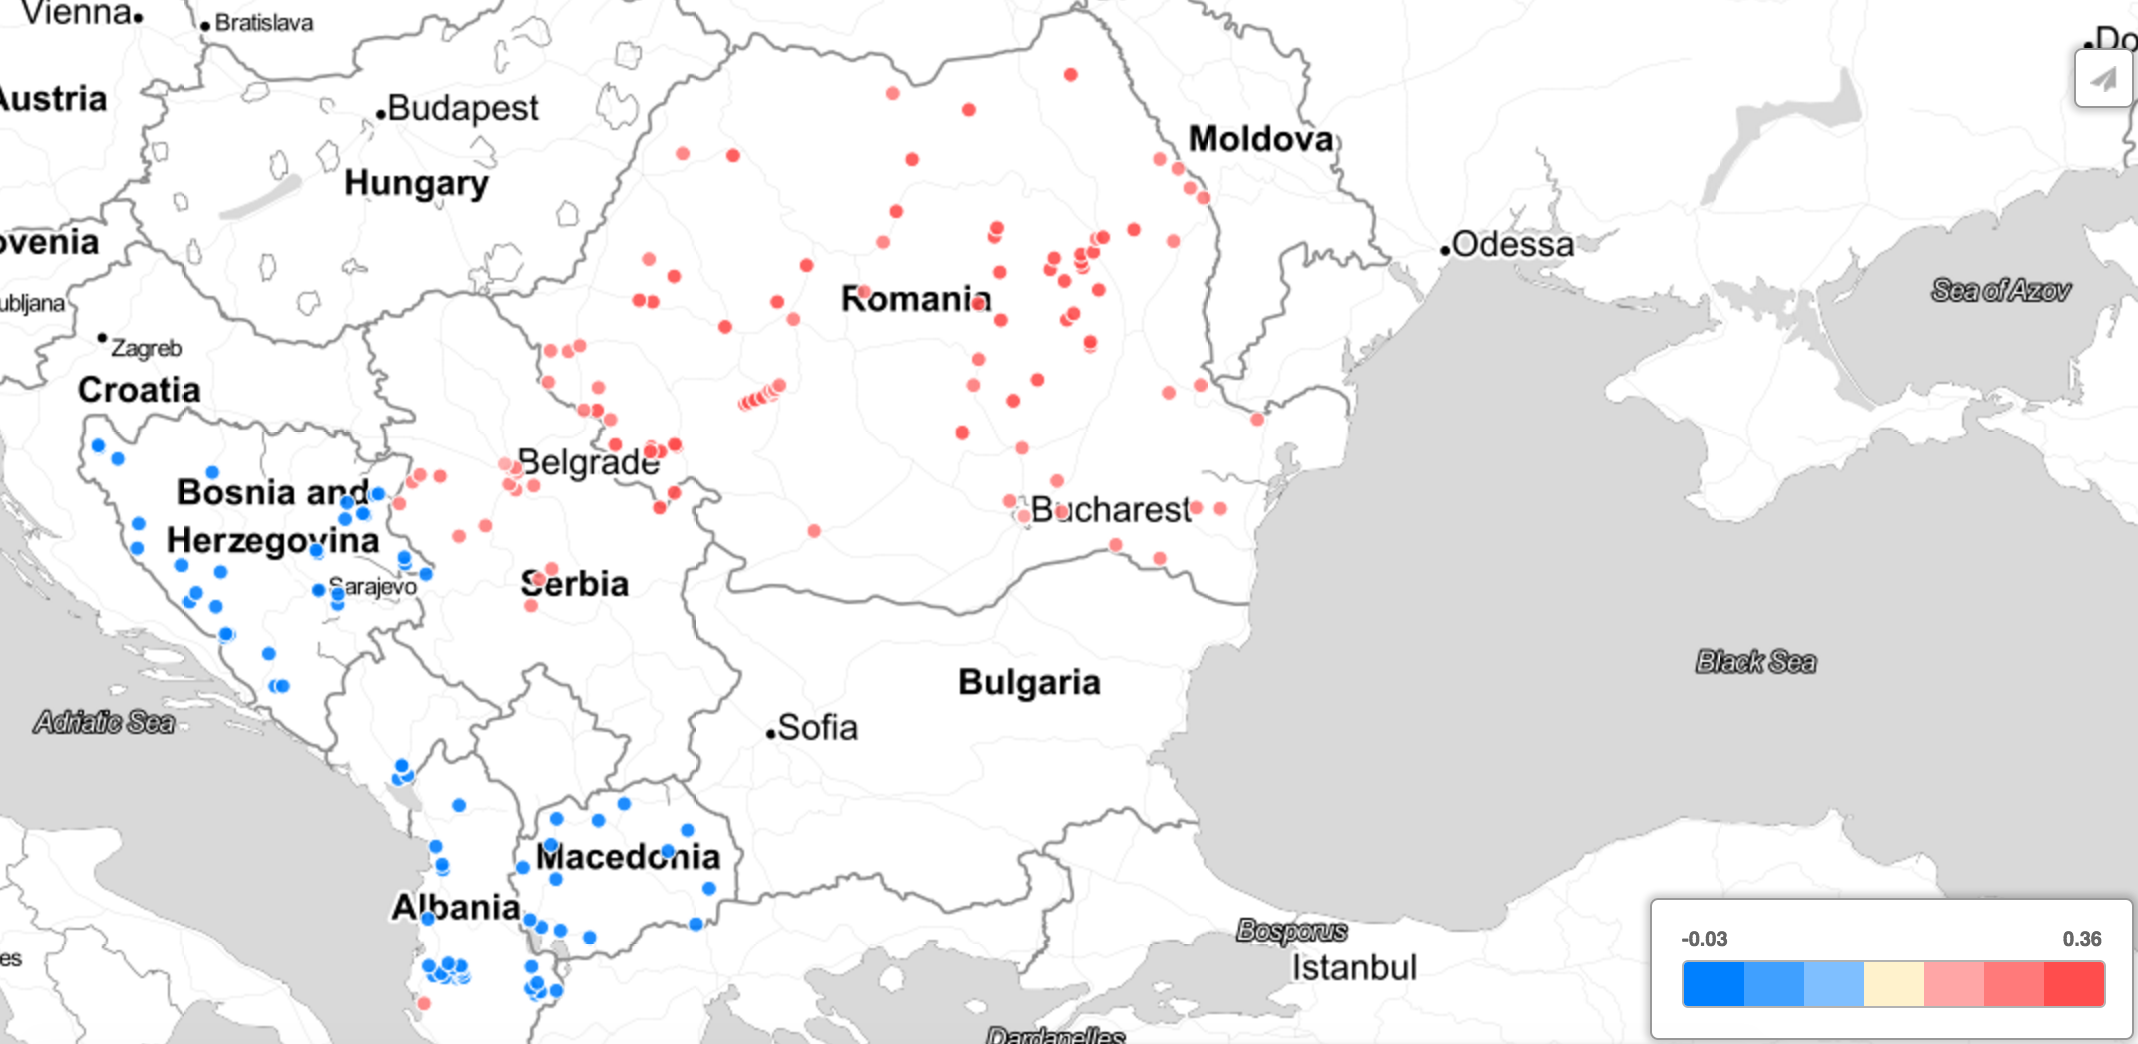
\includegraphics[width=0.35\textwidth]{figs/rfeu.png}\label{figeu:rf}}	
	\subfloat[IEG outcome]{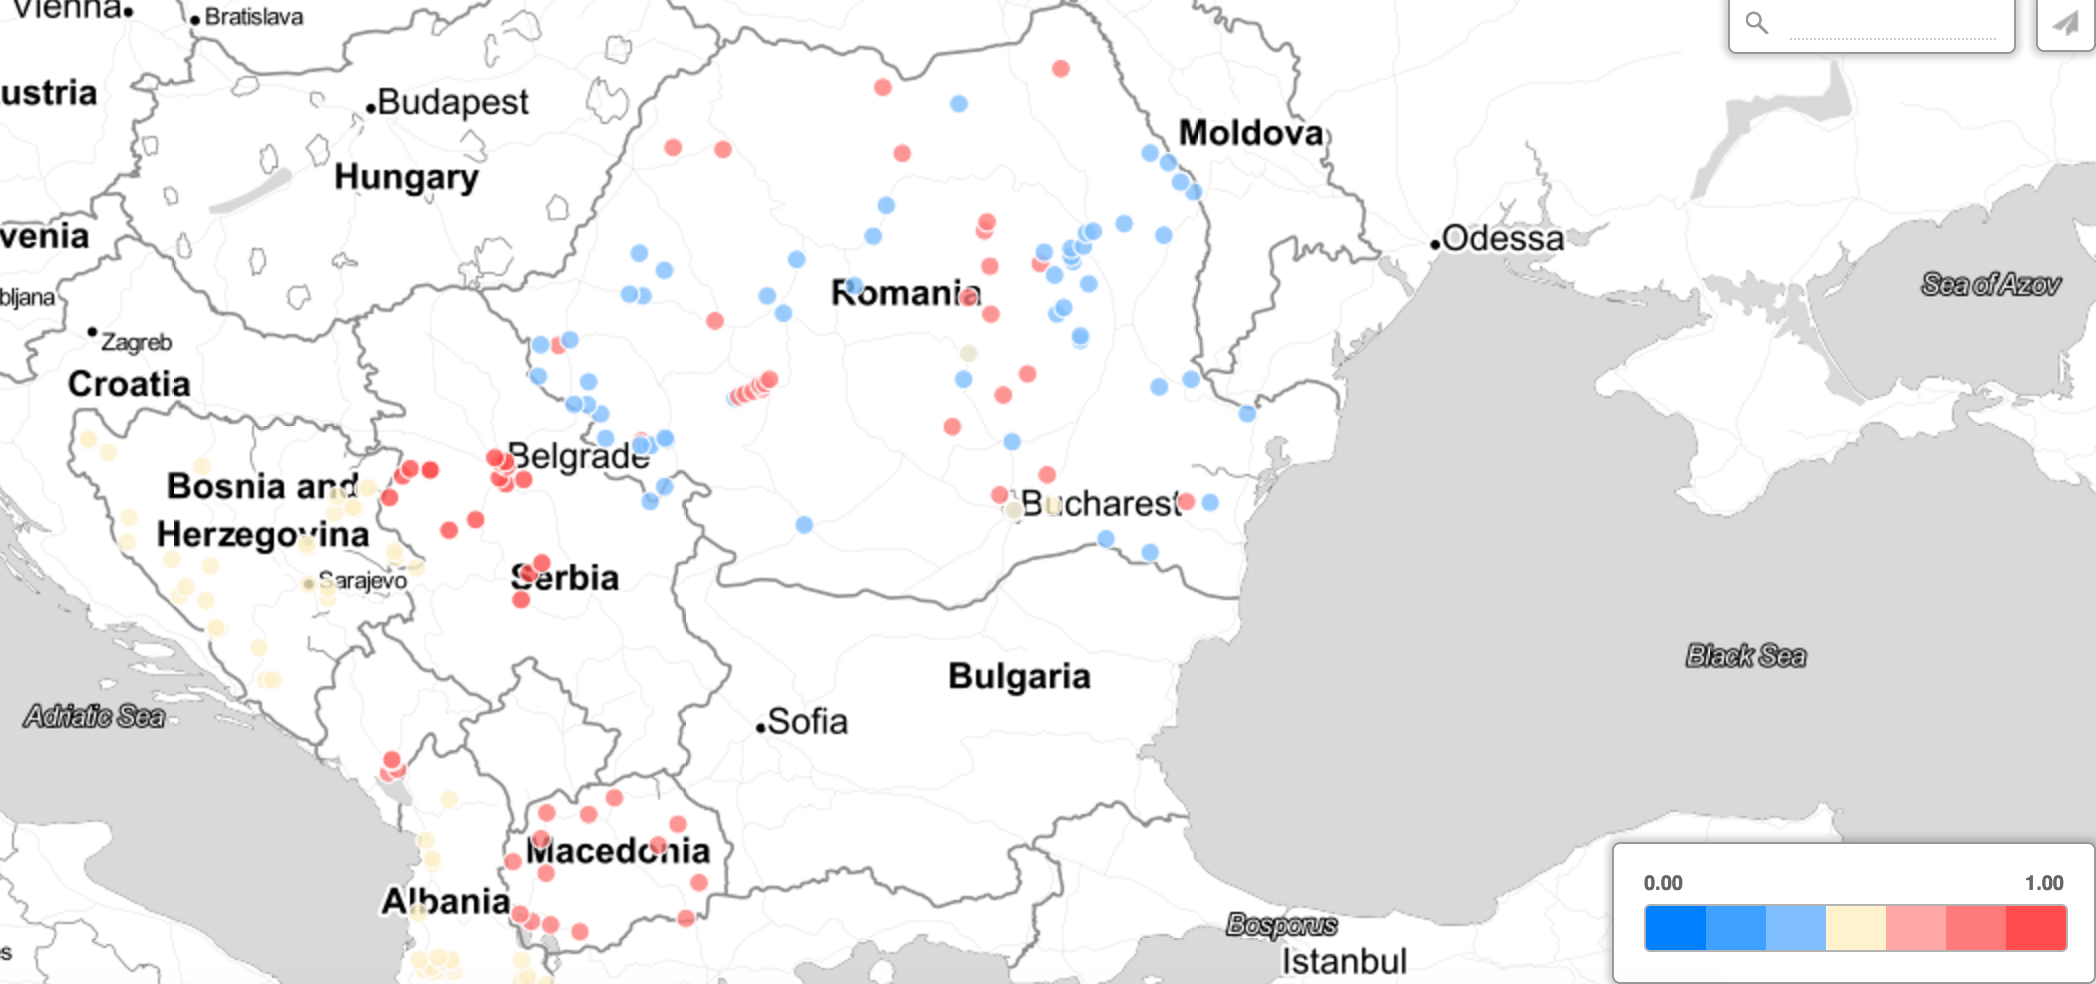
\includegraphics[width=0.35\textwidth]{figs/iegeu.png}\label{figeu:ieg}}
	\caption{East Europe}
\end{figure}



\begin{figure}
	\centering
	\subfloat[CT]{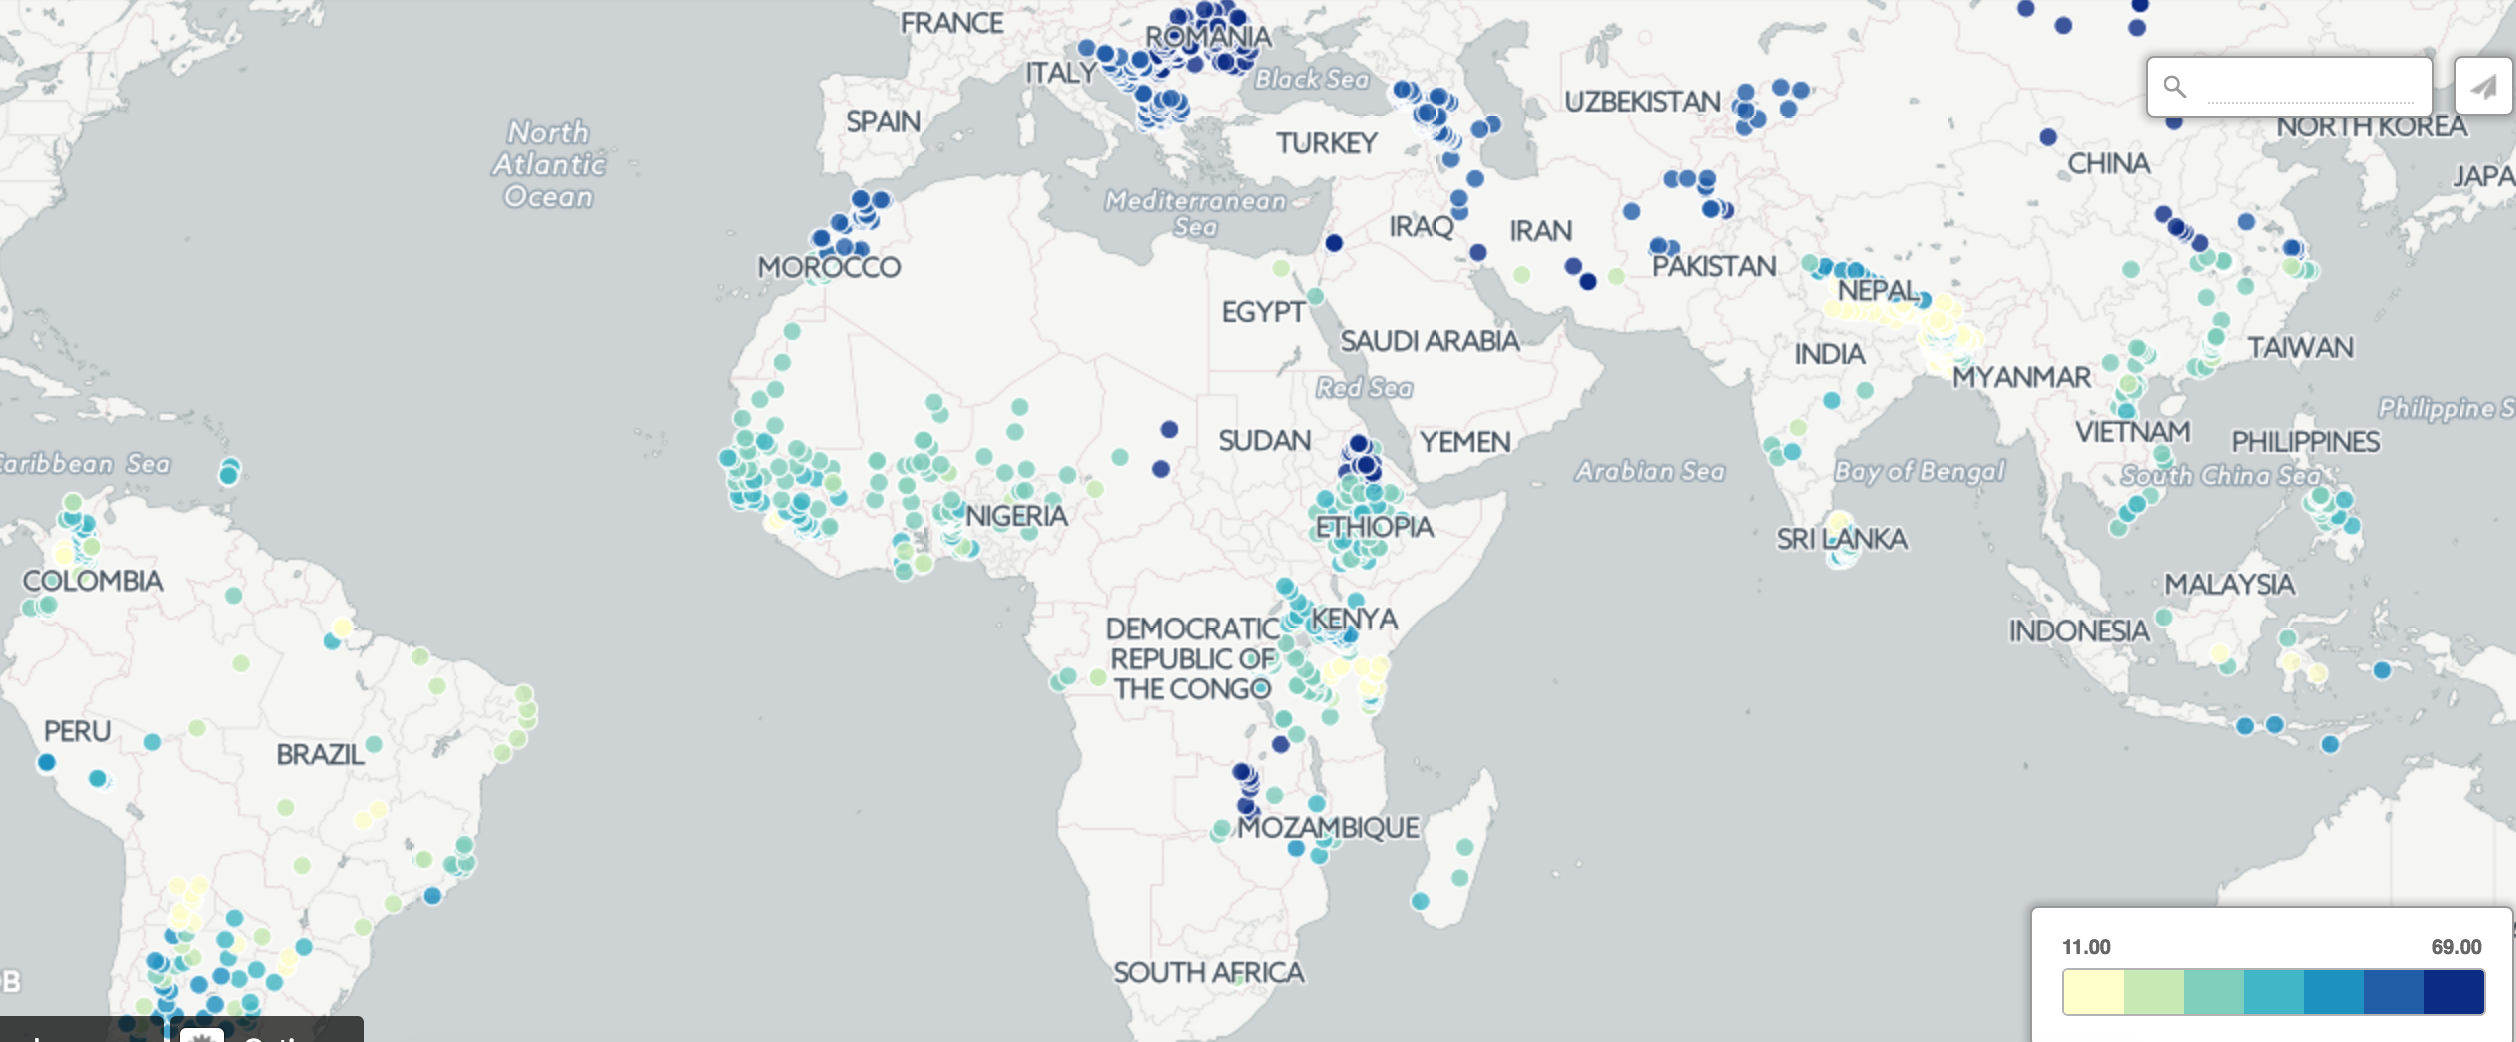
\includegraphics[width=0.5\textwidth]{figs/projectsbyleafct.png}}
	\subfloat[TOT]{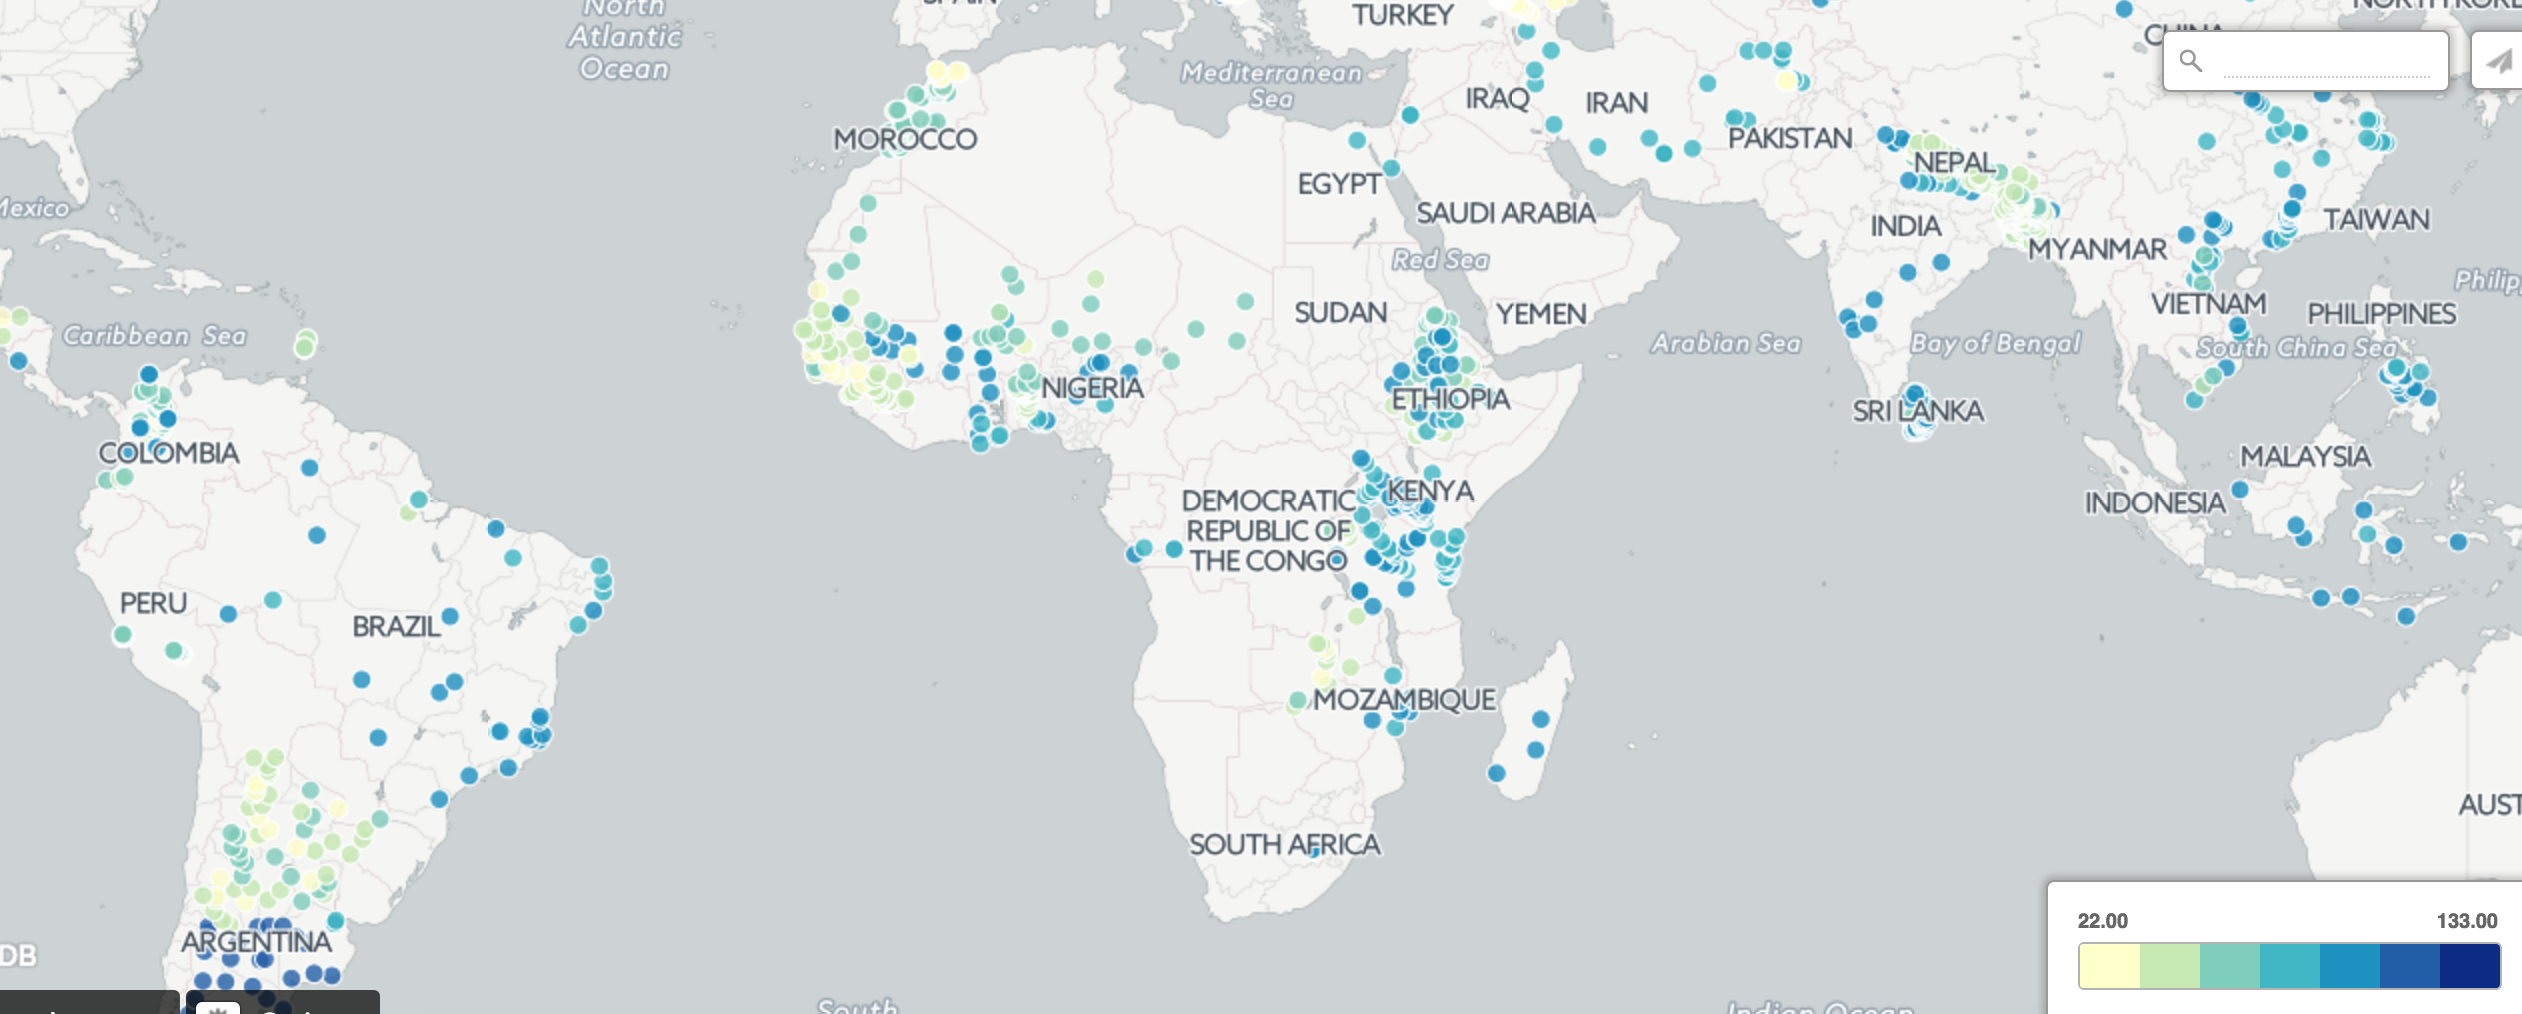
\includegraphics[width=0.5\textwidth]{figs/projectsbyleaftot.png}}
	\label{fig:leaf}
	\caption{projects colored by leaf they fall into }
\end{figure}


\begin{figure}
	\centering
	\subfloat[CT]{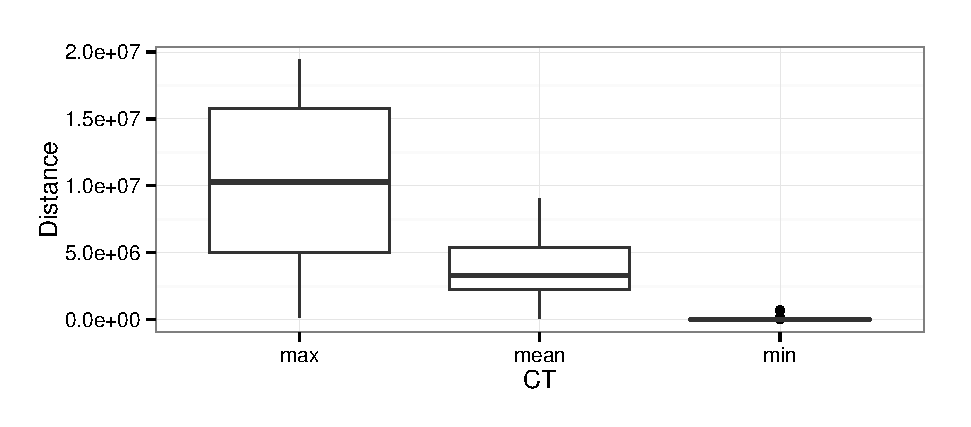
\includegraphics[width=0.5\textwidth]{figs/ctdist.eps}}
	\subfloat[TOT]{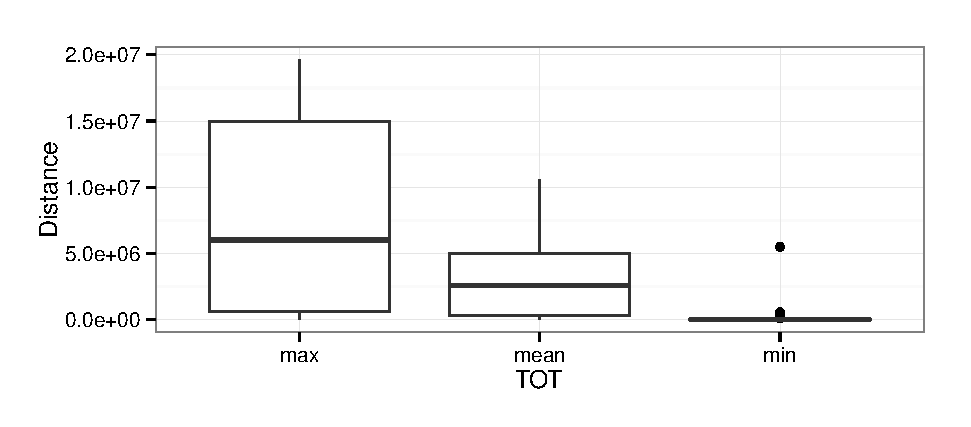
\includegraphics[width=0.5\textwidth]{figs/totdist.eps}}
	\label{fig:leafiest}
	\caption{distance within in the same leaf}
\end{figure}


\subsection{new data set}
Instead of the old data set with time series covariates, we establish the new data set which is the subset of the whole projects, which share the same project starting year, the starting years is between 2000 to 2012, project that started at 2000 has the largest number. We use projects start at 2000 to build the new data set.\\
In the new data set, we transform the time series covariate to the trend before the projects started and the trend after the project started along with the covariates with no time series. Then we use cross validation to choose the optimal complexity parameter and then use it to the new data set. 



\begin{figure}
	\centering
	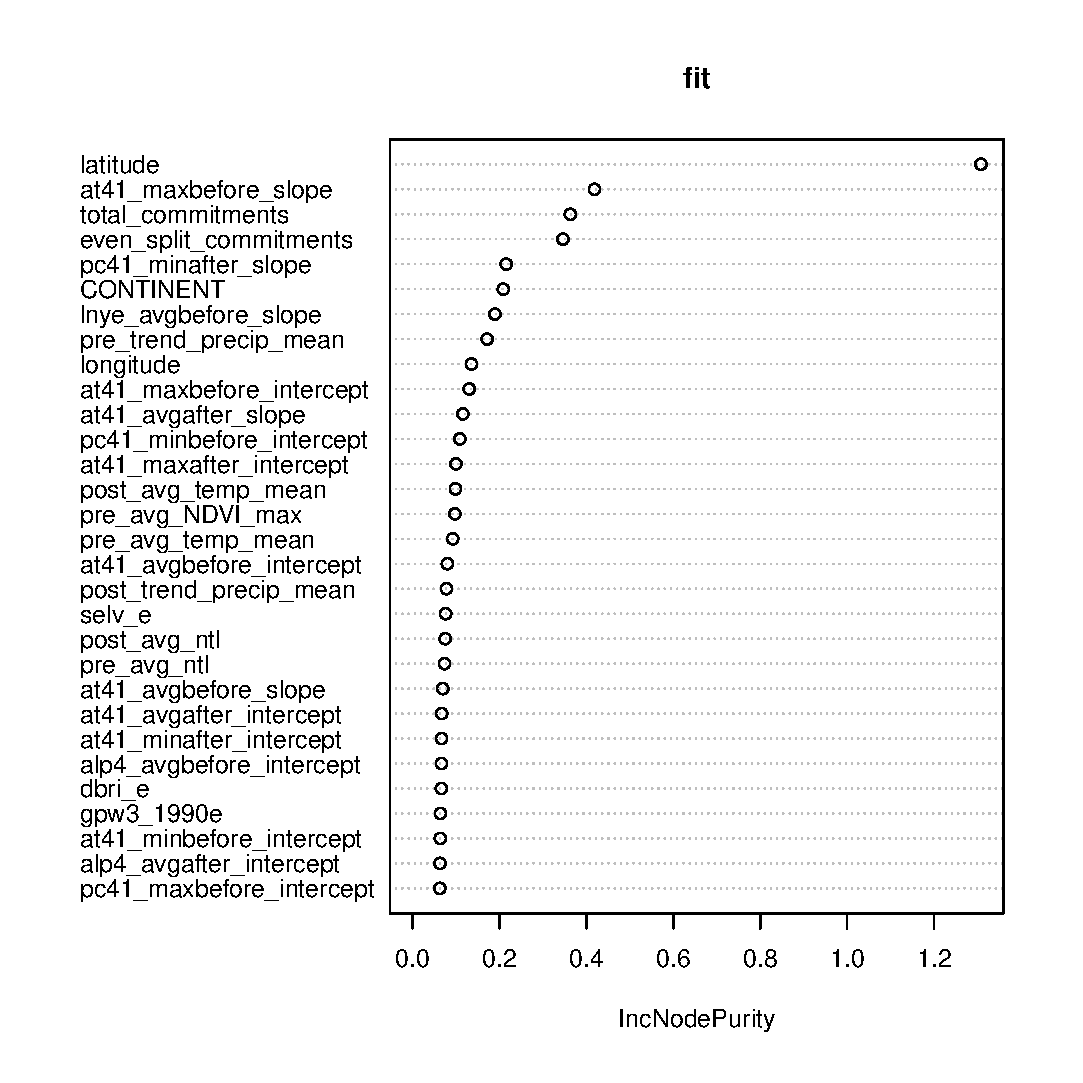
\includegraphics[width=0.6\textwidth]{figs/varimp2004.eps}
	\caption{variable importance 2004 projects}\label{fig:varimp}
\end{figure}

\begin{figure}
	\centering
	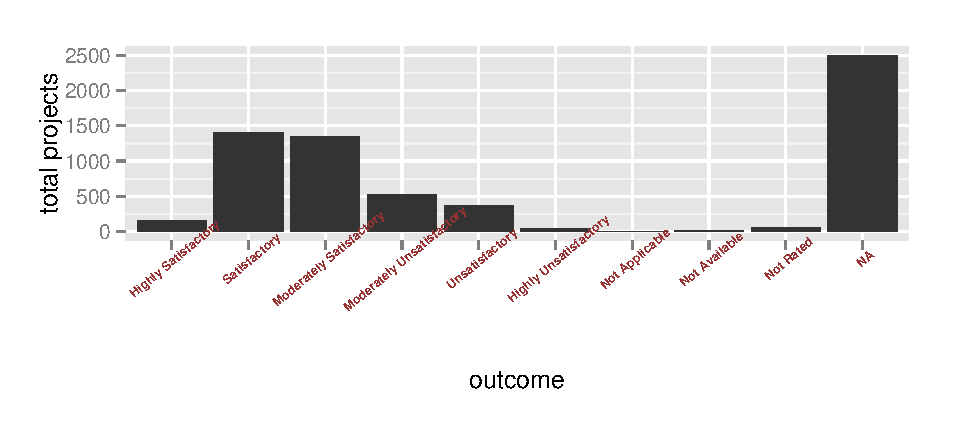
\includegraphics[width=\textwidth]{figs/hist_wb.eps}
	\caption{IEG outcome overview}
\end{figure}


 \begin{figure}
 \centering 
 \includegraphics[page=84,width=0.6\textwidth]{figs/project_2004.pdf}
 \caption{causal tree of projects in 2004}\label{fig:ct}
\end{figure}

\subsection{interpretation of results}
\begin{itemize}
\item Interpretation of data, what can we get out of the random forest?
From the random forest, we can observe the importance of each covariate as shown in \ref{fig:varimp} of year 2004. We can see that latitude is the most important among all the covariates, the other important factors includes the fund of the projects, the max temperature trend before the projects started. 
\item Anecdotal evidence, discuss best and worst project, what is it about, what happens here.

\item Numerical values for CATE? What is the exact interpretation of the calculated values (difficult thanks to propensity score weighting), but estimate of average should have a direct interpretation right? Interpret value for best and worst project.

\item Ranking of projects with respect to CATE?

\item Selection of variables / covariates are commonly selected among trees in the random forest? Provide details, interpret results. E.g. geographic location, show maps.

\item Comparison with an econometric model that looks at carbon foot print(?) Comparison with a world bank project evaluation from a human resources point of view.  In figure \ref{fig:ieg}, take the Nepal area for example, most of the projects are in the medium, neither good nor bad from the IEG outcome. In the random forest model, in figure \ref{fig:rf}, blue points are project in Nepal and the red points are projects in India, from this model, the cause effect in India is better that projects in Nepal, random forest model and economist model both have negative causal effect in Nepal, the difference between these two models is that projects have negative effect by economist model, but good effect by the random forest model. (what's the shortcoming of the econ model? ) In Nepal, the projects from the title are eduction and poverty alleviation projects, while in India they are Uttaranchal Decentralized Watershed project(how to explain?)Another example is the east Europe example, in both the random forest and economist model, they estimate Romain and Serbia projects achieve good effect while the effect is bigger in the random forest model than that in the economist model.In the IEG outcome, they evaluate the projects as moderate or unsatisfactory. The projects are Transport Restructuring Project, Mine Closure, Environment and Socio-Economic Regeneration Project, Modernizing Agricultural Knowledge and Information Systems Project (MAKIS).
In Bosnia and Herzegovina, random forest evaluate the projects has negative effect while the econ model rate them as positive, the projects title is Urban Infrastructure and Service Delivery Project. (No idea if these projects will cut trees or not or something else related with NDVI). The IEG outcome is Moderately Unsatisfactory for projects in this country. 


\item What do projects fall into the same leaf in the tree show in the map? In \ref{fig:leaf}, we can observe that both causal tree and transformed outcome tree would group projects nearby together, and we believe geographic information has big impact to the causal effect, which also in consistent with the important variable in the random forest. 

\end{itemize}

\section{related work}
Causality \cite{Pearl:2000:CMR:331969} plays an important role in many area. In this paper, we focus on the heterogeneous causal effects.
Some paper in the literature use tree based machine learning technique to estimate heterogeneous causal effects.
In \cite{journals/jmlr/SuTWNL09}, they use statistical test as the criterion for node splitting.  In \cite{1504.01132}, they use causal trees to estimate heterogeneous treatment effect. However, they do not show what if in some nodes, there is only treated units or only untreated units and then how to estimate the heterogeneous causal effects.\\
Some paper use forest based machine learning technique to estimate heterogeneous causal effects. In \cite{1510.04342}, they use casual forest to do heterogeneous causal effects estimation, and they share the same idea in paper \cite{Denil:2014} that they use difference data for the structure of the tree and the estimation value within each node.

\section{Conclusions}
issues: number of control units in leaves

precision of answers

robustness of random forest for TOT

spill over effect in spatial data (big project next to untreated case)

spatial diversity in leaf nodes (not just diversity in values)
\bibliographystyle{splncs03}
\bibliography{bibtex}

\end{document}
